%!TEX root = ../main.tex
\chapter{Leggi di conservazioni scalari}

Sono equazioni differenziali del tipo
\begin{equation}
    u=u(x,t) \ \ \ \ \boxed{u_{t} +q(u)_{x} =0}\ \ x\in \mathbb{R} ,\ t >0
\end{equation}
\textbf{se }$q$\textbf{ e }$u$\textbf{ sono regolari}, per la regola della catena $q(u)_{x} =q'(u) \cdotp u_{x}$.
\begin{itemize}
    \item $u$ è da pensare come concentrazione di una sostanza (massa su lunghezza per esempio)
    \item $\mathbf{q}$ è il vettore di flusso, mentre $q(u)$ funzione di flusso.
          \begin{equation}
              \mathbf{q} =q(u)\mathbf{i}
          \end{equation}
\end{itemize}

Se consideriamo un tratto dell'ipotetico canale dove stiamo studiando la concentrazione, la variazione nel tempo della massa è data dalla differenza tra il flusso agli estremi, ed una eventuale sorgente
\begin{equation*}
    \frac{\de}{\dt}\int ^{x_{2}}_{x_{1}} u(y,t) \dy=q(u(x_{1} ,t)) -q(u(x_{2} ,t)) +\underbrace{\left(\int ^{x_{2}}_{x_{1}} f(y,t) \dy\right)}_{\text{sorgente non omogenea}}
\end{equation*}
\emph{Nel caso in cui fosse possibile passare sotto il segno di integrale}, l'integrale diventa:
\begin{equation}
    \frac{\de}{\dt}\int ^{x_{2}}_{x_{1}} u(y,t) \dy=\int ^{x_{2}}_{x_{1}} u_{t}(y,t) \dy
    \label{eq:lc-passaggio-derivata-integrale}
\end{equation}
mentre l'altro termine si può scrivere naturalmente come\footnote{Teorema fondamentale del calcolo integrale.}
\begin{equation*}
    -q(u(x_{1} ,t)) +q(u(x_{2} ,t)) =\int ^{x_{2}}_{x_{1}} q(u)_{x} \dx
\end{equation*}
che per arbitrarietà dell'intervallo implica proprio la legge di conservazione:
\begin{equation*}
    \int ^{x_{2}}_{x_{1}}[ u_{t} +q(u)_{x}] \dx=0,\ \forall x_{1} ,x_{2} \ \ \Rightarrow \ \ u_{t} +q(u)_{x} =0
\end{equation*}
Capito il contesto, dobbiamo scegliere con quale $q$ decidiamo di lavorare, in altre parole dobbiamo scegliere una legge costitutiva per $q$.

Consideriamo in particolare il \textbf{trasporto lineare}, anche se in generale la dipendenza da $u$ è non lineare (vedremo più avanti modelli per questi casi). Nel trasporto lineare, $q$ è fatta come segue, con $v$ costante
\begin{equation}
    q(u) =vu
\end{equation}
da cui $q(u)_{x} =vu_{x}$.

L'equazione differenziale si scrive nei due casi
\begin{itemize}
    \item \textbf{omogeneo}
          \begin{equation*}
              \begin{cases}
                  u_{t} +vu_{x} =\boxed{0} & \text{in} \ \mathbb{R} \times (0,+\infty) \\
                  u(x,0) =g(x)             & \text{in} \ \mathbb{R}
              \end{cases}
          \end{equation*}
    \item \textbf{non omogeneo}
          \begin{equation*}
              \begin{cases}
                  u_{t} +vu_{x} =\boxed{f(x,t)} & \text{in} \ \mathbb{R} \times (0,+\infty) \\
                  u(x,0) =g(x)                  & \text{in} \ \mathbb{R}
              \end{cases}
          \end{equation*}
\end{itemize}
\section{Caso omogeneo}

Introduciamo il vettore $\mathbf{w} =v\mathbf{i} +\mathbf{j}$, allora l'equazione differenziale si può scrivere come
\begin{equation*}
    0=u_{t} +vu_{x} =
    \begin{pmatrix}
        u_{x} & u_{t}
    \end{pmatrix} \cdotp \begin{pmatrix}
        v \\
        1
    \end{pmatrix} =\nabla u\cdotp \mathbf{w}
\end{equation*}
ma il gradiente $\nabla u$ è per proprietà sempre ortogonale alle linee di livello di $u$, ovvero i valori in cui è costante, date da
\begin{equation*}
    \left\{x:u(x,t) =\text{costante per un tempo fissato}\right\}
\end{equation*}
poiché $\mathbf{w}$ è costante, \textbf{le linee di livello sono rette nella direzione} $\mathbf{w}$:
\begin{equation}
    x=vt+x_{0}
\end{equation}
Su tali rette $u$ è costante e le chiamiamo \textbf{rette caratteristiche.}

Per risolvere il problema di Cauchy, si calcola $u$ in $(\overline{x} ,\overline{t})$ nel seguente modo

\fg[Caratteristica del trasporto lineare.]{0.4}{leggi-conservazione-caratteristica-trasporto-lineare}

calcoliamo la retta caratteristica per quel punto e la mandiamo indietro nel tempo finché non incontra l'asse $x$ su tale retta $u$ è costante e uguale al dato iniziale $g(x_{0})$
\begin{equation*}
    u(\overline{x} ,\overline{t}) =g(x_{0}) =g(x-vt)
\end{equation*}
In conclusione, la soluzione del problema di Cauchy è data da
\begin{equation}
    u(x,t) =g(x-vt)
\end{equation}
questa è un'\textit{onda progressiva}, viaggiante, che si muove verso destra con velocità $v$.

\fg[Onda progressiva.]{0.5}{leggi-conservazione-onda-progressiva}

Il profilo di $u$ si mantiene inalterato. In generale la regola del segno è
\begin{equation*}
    u_{t} \pm vu_{x} =0\ \ \Rightarrow \ \ g(x\mp vt)
\end{equation*}
\section{Caso non omogeneo}
\label{sec:leggi-conservazione-non-omogeneo}

Non possiamo aspettarci che lungo la caratteristica $u$ sia costante, ciò nonostante consideriamo una caratteristica e consideriamo come varia in funzione di $t$ denotando una nuova funzione $w$
\begin{equation*}
    u(x,t) = u(vt+x_{0} ,t) =w(t)
\end{equation*}
andiamo a calcolare $w'$, che dovrà essere uguale a $f$ sulla caratteristica
\begin{equation*}
    w'(t) =u_{t}(vt+x_{0} ,t) +u_{x}(vt+x_{0} ,t) \cdotp v=f(vt+x_{0} ,t)
\end{equation*}
abbiamo l'equazione differenziale per $w$
\begin{equation*}
    \begin{cases}
        w'(t) =f(vt+x_{0} ,t) \\
        w(0) =g(x_{0})
    \end{cases}
\end{equation*}
qui si può mettere tranquillamente il pilota automatico e dire che
\begin{equation*}
    w(t) =g(x_{0}) +\int ^{t}_{0} f(vs+x_{0} ,s) \ds
\end{equation*}
tornando ad $u$, notiamo che $vs+x_{0}=vs+x-vt=x-v(t-s)$
\begin{equation}
    u(x,t) =g(x-vt) +\int ^{t}_{0} f(x-v(t-s) ,s) \ds
\end{equation}
è la soluzione se $g\in C^{1}(\mathbb{R})$ e $f,f_{x} \in C(\mathbb{R} \times [ 0,+\infty))$. Si può confrontare facilmente col caso omogeneo e notare che il risultato è il medesimo se $f=0$.

\section{Modelli di dinamica del traffico}

Studiamo il traffico lungo un tratto rettilineo (autostrada per esempio), visto da molto in alto, come un fluido in movimento, descritto da $3$ variabili
\begin{itemize}
    \item $\rho $ densità di auto (auto/km), la nostra incognita
    \item $v$ velocità media delle auto (km/tempo)
    \item $q$ funzione di flusso (auto/tempo)
\end{itemize}
Per le ultime due avremo bisogno di relazioni costitutive.

Ipotesi di base
\begin{itemize}
    \item una sola corsia, senza sorpassi
    \item assenza di caselli (assenza di \textit{sorgenti} o \textit{pozzi} di auto), quindi problema \emph{omogeneo}
    \item la velocità è funzione di $\rho $, cioè $v=v(\rho)$, è un'ipotesi un po' controversa perché bisognerebbe considerare un tempo di reazione dei guidatori. Se aumenta la densità diminuisce la velocità $\frac{\dv}{\drho} \leq 0$.
\end{itemize}

Abbiamo
\begin{equation}
    \begin{cases}
        \rho _{t} +q(\rho)_{x} =0 & x\in \mathbb{R} ,\ t >0 \\
        \rho (x,0) =g(x)          & x\in \mathbb{R}
    \end{cases}
\end{equation}

\textbf{Legge costitutiva per} $q$.
Nell'ipotesi di trasporto convettivo (senza diffusione)
\begin{equation}
    q=\rho v
\end{equation}

\textbf{Legge costitutiva per} $v$.
Prendiamo la legge più semplice, ci saranno
\begin{itemize}
    \item $v_{m}$ velocità massima
    \item $\rho _{m}$ densità massima
\end{itemize}

ci aspettiamo che
\begin{equation*}
    v(0) =v_{m} \ \ \ \ v(\rho _{m}) =0
\end{equation*}
il modello più semplice è l'interpolazione lineare che realizza queste due condizioni
\begin{equation}
    v(\rho) =v_{m}\left(1-\frac{\rho }{\rho _{m}}\right)
\end{equation}


\begin{figure}[H]
    \centering

    \tikzset{every picture/.style={line width=0.75pt}} %set default line width to 0.75pt        


    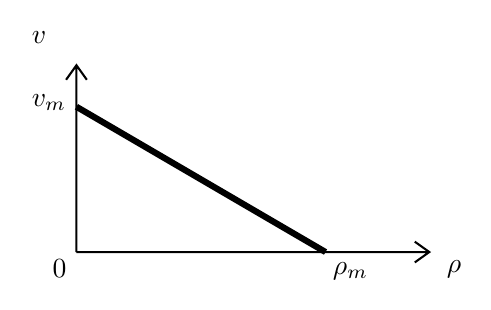
\begin{tikzpicture}[x=0.75pt,y=0.75pt,yscale=-1,xscale=1]
        %uncomment if require: \path (0,140); %set diagram left start at 0, and has height of 140

        %Shape: Axis 2D [id:dp9160346144505975] 
        \draw  (220,110) -- (390,110)(220,20) -- (220,110) -- cycle (383,105) -- (390,110) -- (383,115) (215,27) -- (220,20) -- (225,27)  ;
        %Straight Lines [id:da4398967911531251] 
        \draw [line width=2.25]    (220,40) -- (340,110) ;

        % Text Node
        \draw (197,2.4) node [anchor=north west][inner sep=0.75pt]    {$v$};
        % Text Node
        \draw (397,112.4) node [anchor=north west][inner sep=0.75pt]    {$\rho $};
        % Text Node
        \draw (342,113.4) node [anchor=north west][inner sep=0.75pt]    {$\rho _{m}$};
        % Text Node
        \draw (197,32.4) node [anchor=north west][inner sep=0.75pt]    {$v_{m}$};
        % Text Node
        \draw (207,112.4) node [anchor=north west][inner sep=0.75pt]    {$0$};

    \end{tikzpicture}

\end{figure}
\FloatBarrier

di conseguenza
\begin{equation*}
    q(\rho) =\rho v(\rho)=v_{m}\left(\rho -\frac{\rho ^{2}}{\rho _{m}}\right) \ \ \Rightarrow \ \ q'(\rho) =v_{m}\left(1-\frac{2\rho }{\rho _{m}}\right) \ \ \Rightarrow \ \ q''(\rho) =-\frac{2v_{m}}{\rho _{m}} < 0
\end{equation*}
da cui
\begin{equation*}
    \begin{cases}
        \rho _{t} +\underbrace{v_{m}\left(1-\frac{2\rho }{\rho _{m}}\right)}_{q'(\rho)} \rho _{x} =0 & x\in \mathbb{R} ,\ t >0 \\
        \rho (x,0) =g(x)                                                                             & x\in \mathbb{R}
    \end{cases}
\end{equation*}
Cerchiamo di imitare il metodo delle caratteristiche.

Idea: dato $(x,t)$ determinare una linea $x=x(t)$ lungo la quale $\rho $ sia costante, che connetta $(x,t)$ ad un punto $(x_{0} ,0)$

\fg{0.4}{leggi-conservazione-traffico-caratteristica}

Se tutto va in porto allora $\rho (x,t) =g(x_{0})$.

\textbf{Il problema sarà se riusciremo ad esprimere $x_{0}$ in funzione di $x,t$} così da ottenere qualcosa di generale. Notiamo anche che non sappiamo nemmeno se sarà una retta.

Imponiamo che lungo $x=x(t)$, $\rho $ sia costante
\begin{equation}
    \rho (x(t) ,t) =g(x_{0})
    \label{eq:lc-ro-costante}
\end{equation}
deriviamo nel tempo
\begin{equation*}
    \rho _{t}(x(t) ,t) +\dot{x}(t) \cdotp \rho _{x}(x(t) ,t) =0
\end{equation*}
ho anche l'equazione differenziale, valutata lungo la curva, imponendo \eqref{eq:lc-ro-costante}
\begin{align*}
    \rho _{t}(x(t) ,t) +q'(\textcolor[rgb]{0.82,0.01,0.11}{\rho (x(t) ,t)}) \rho _{x}(x(t) ,t) & =0 \\
    \rho _{t}(x(t) ,t) +q'(\textcolor[rgb]{0.82,0.01,0.11}{g(x_{0})}) \rho _{x}(x(t) ,t)       & =0
\end{align*}
sottraggo
\begin{equation*}
    [\dot{x}(t) -q'(g(x_{0}))] \rho _{x}(x(t) ,t) =0
\end{equation*}
ma $\rho _{x} =0$ non è ragionevole\footnote{Se lo fosse, allora la PDE si ridurrebbe a $\rho _{t}=0$, ovvero la soluzione sarebbe costante ovunque. Se già il dato iniziale non è costante, è chiaro che ciò non può tornare.}, quindi
\begin{equation*}
    \begin{cases}
        \dot{x}(t) =q'(g(x_{0})) \\
        x(0) =x_{0}
    \end{cases}
\end{equation*}
quindi le equazioni delle caratteristiche \textbf{sono ancora rette}, ma il coefficiente angolare dipende dal dato iniziale. Si noti che solitamente esprimiamo $x$ in funzione di $t$, mentre i grafici hanno nelle ascisse $x$ e nelle ordinate $t$, al contrario di come usualmente si fa. Nel pensare alla \emph{pendenza} del grafico bisogna quindi fare riferimento alle ordinate.
\begin{equation}
    x=q'(g(x_{0})) t+x_{0}
\end{equation}
Il punto è quindi determinare $x_{0}$ in funzione dei generici $x,t$, per poi tornare a $\rho $ in \eqref{eq:lc-ro-costante}
\begin{equation}
    \rho (x,t) =g(x_{0}) =g(x-q'(g(x_{0})) t)
    \label{eq:lc-sol-ro-traffico}
\end{equation}
è ancora un'onda progressiva, ma la velocità non è costante con $x_{0}$, infatti $q'(g(x_{0}))$ si chiama \textbf{velocità locale dell'onda}. È la velocità di un segnale che si propaga, non del traffico.

Si noti infatti che:
\begin{equation*}
    \underbrace{q'(\rho)}_{\text{vel.segnale}} = \frac{\de}{\drho}q(\rho) = \frac{\de}{\drho}(\rho v) = \underbrace{\frac{\drho }{\drho }}_{=1}v + \rho \underbrace{\frac{\de v}{\drho}}_{\le 0} \le \underbrace{v}_{\text{vel.traffico}}
\end{equation*}

Notiamo anche che in questo modello di traffico la velocità delle macchine sarà sempre maggiore o uguale a zero, mentre disegnando il grafico di $q'(\rho $ ci si rende facilmente conto che la velocità locale dell'onda può facilmente essere negativa (un segnale che si propaga all'indietro, come vedremo nell'esempio della coda al semaforo).

Problema: \eqref{eq:lc-sol-ro-traffico} dà sempre soluzione? No.

\fg{0.4}{leggi-conservazione-shock}

Se due caratteristiche si intersecano, il valore \textbf{nell'intersezione non è determinato}: sono in presenza di un'ambiguità. Motiviamo con due esempi.
\subsection{Coda al semaforo}

Modellizziamo il problema come

\fg{0.4}{leggi-conservazione-coda-semaforo}
Abbiamo già tutto il modello pronto, dobbiamo solo scegliere il dato iniziale
\begin{equation}
    g(x) =
    \begin{cases}
        \rho _{m} & x< 0 \\
        0         & x >0
    \end{cases}
\end{equation}
Una possibile strategia è:
\begin{enumerate}
    \item Calcolare la velocità locale dell'onda $q'(g(x_{0}))$ al variare di $x_{0}$;
    \item Determinare e tracciare nel piano $(x,t)$ le caratteristiche;
    \item Calcolare la soluzione $\rho (x,t)$.
\end{enumerate}

A $t=0$ il semaforo diventa verde, come evolve il traffico? Ci aspettiamo che le macchine davanti al semaforo si inizino a muovere velocità massima, le altre rimangono un po' ferme e poi partano.
\begin{enumerate}
    \item Velocità locale dell'onda, ricordiamo che
          \begin{equation*}
              q'(\rho) =v_{m}\left(1-\frac{2\rho }{\rho _{m}}\right)
          \end{equation*}

          dobbiamo distinguere per i due valori di $\rho $
          \begin{equation*}
              q'(g(x_{0})) =
              \begin{cases}
                  -v_{m} & x_{0} < 0 \\
                  v_{m}  & x_{0}  >0
              \end{cases}
          \end{equation*}
    \item Le caratteristiche sono
          \begin{equation*}
              \begin{cases}
                  x=-v_{m} t+x_{0} & x_{0} < 0 \\
                  x=v_{m} t+x_{0}  & x_{0}  >0
              \end{cases}
          \end{equation*}
          \begin{figure}[htpb]
              \centering


              \tikzset{every picture/.style={line width=0.75pt}} %set default line width to 0.75pt        

              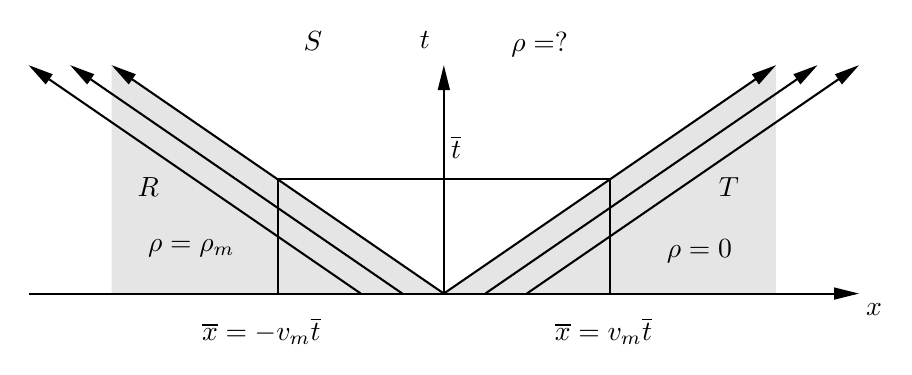
\begin{tikzpicture}[x=0.75pt,y=0.75pt,yscale=-1,xscale=1]
                  %uncomment if require: \path (0,300); %set diagram left start at 0, and has height of 300

                  %Straight Lines [id:da31860563022767274] 
                  \draw    (30,160) -- (428,160) ;
                  \draw [shift={(430,160)}, rotate = 180] [fill={rgb, 255:red, 0; green, 0; blue, 0 }  ][line width=0.08]  [draw opacity=0] (12,-3) -- (0,0) -- (12,3) -- cycle    ;
                  %Straight Lines [id:da03734817952352376] 
                  \draw    (230,160) -- (230,52) ;
                  \draw [shift={(230,50)}, rotate = 450] [fill={rgb, 255:red, 0; green, 0; blue, 0 }  ][line width=0.08]  [draw opacity=0] (12,-3) -- (0,0) -- (12,3) -- cycle    ;
                  %Straight Lines [id:da7275304597797716] 
                  \draw    (230,160) -- (388.35,51.13) ;
                  \draw [shift={(390,50)}, rotate = 505.49] [fill={rgb, 255:red, 0; green, 0; blue, 0 }  ][line width=0.08]  [draw opacity=0] (12,-3) -- (0,0) -- (12,3) -- cycle    ;
                  %Straight Lines [id:da5312343881098429] 
                  \draw    (250,160) -- (408.35,51.13) ;
                  \draw [shift={(410,50)}, rotate = 505.49] [fill={rgb, 255:red, 0; green, 0; blue, 0 }  ][line width=0.08]  [draw opacity=0] (12,-3) -- (0,0) -- (12,3) -- cycle    ;
                  %Straight Lines [id:da1295802157961734] 
                  \draw    (270,160) -- (428.35,51.13) ;
                  \draw [shift={(430,50)}, rotate = 505.49] [fill={rgb, 255:red, 0; green, 0; blue, 0 }  ][line width=0.08]  [draw opacity=0] (12,-3) -- (0,0) -- (12,3) -- cycle    ;
                  %Straight Lines [id:da529793434413488] 
                  \draw    (230,160) -- (71.65,51.13) ;
                  \draw [shift={(70,50)}, rotate = 394.51] [fill={rgb, 255:red, 0; green, 0; blue, 0 }  ][line width=0.08]  [draw opacity=0] (12,-3) -- (0,0) -- (12,3) -- cycle    ;
                  %Straight Lines [id:da78569330537292] 
                  \draw    (210,160) -- (51.65,51.13) ;
                  \draw [shift={(50,50)}, rotate = 394.51] [fill={rgb, 255:red, 0; green, 0; blue, 0 }  ][line width=0.08]  [draw opacity=0] (12,-3) -- (0,0) -- (12,3) -- cycle    ;
                  %Straight Lines [id:da45836696796825693] 
                  \draw    (190,160) -- (31.65,51.13) ;
                  \draw [shift={(30,50)}, rotate = 394.51] [fill={rgb, 255:red, 0; green, 0; blue, 0 }  ][line width=0.08]  [draw opacity=0] (12,-3) -- (0,0) -- (12,3) -- cycle    ;
                  %Shape: Rectangle [id:dp18140614611860273] 
                  \draw   (150,105) -- (310,105) -- (310,160) -- (150,160) -- cycle ;
                  %Shape: Right Triangle [id:dp6794336263527512] 
                  \draw  [draw opacity=0][fill={rgb, 255:red, 0; green, 0; blue, 0 }  ,fill opacity=0.1 ] (70,50) -- (230,160) -- (70,160) -- cycle ;
                  %Shape: Right Triangle [id:dp9252510934255156] 
                  \draw  [draw opacity=0][fill={rgb, 255:red, 0; green, 0; blue, 0 }  ,fill opacity=0.1 ] (390,50) -- (230,160) -- (390,160) -- cycle ;

                  % Text Node
                  \draw (81,102.4) node [anchor=north west][inner sep=0.75pt]    {$R$};
                  % Text Node
                  \draw (361,102.4) node [anchor=north west][inner sep=0.75pt]    {$T$};
                  % Text Node
                  \draw (161,32.4) node [anchor=north west][inner sep=0.75pt]    {$S$};
                  % Text Node
                  \draw (217,32.4) node [anchor=north west][inner sep=0.75pt]    {$t$};
                  % Text Node
                  \draw (232,82.4) node [anchor=north west][inner sep=0.75pt]    {$\overline{t}$};
                  % Text Node
                  \draw (432,163.4) node [anchor=north west][inner sep=0.75pt]    {$x$};
                  % Text Node
                  \draw (336,132.4) node [anchor=north west][inner sep=0.75pt]    {$\rho =0$};
                  % Text Node
                  \draw (86,132.4) node [anchor=north west][inner sep=0.75pt]    {$\rho =\rho _{m}$};
                  % Text Node
                  \draw (261,32.4) node [anchor=north west][inner sep=0.75pt]    {$\rho =?$};
                  % Text Node
                  \draw (282,170.4) node [anchor=north west][inner sep=0.75pt]    {$\overline{x} =v_{m}\overline{t}$};
                  % Text Node
                  \draw (112,170.4) node [anchor=north west][inner sep=0.75pt]    {$\overline{x} =-v_{m}\overline{t}$};

              \end{tikzpicture}
          \end{figure}
          \FloatBarrier

    \item Le rette $x=\pm v_{m}t$ delimitano $3$ settori: $R,S,T$
          \begin{equation*}
              \begin{cases}
                  \text{in} \ R:\ \ x< -v_{m} t & \Rightarrow \ \ \rho =\rho _{m} \\
                  \text{in} \ T:\ \ x >v_{m} t  & \Rightarrow \ \ \rho =0
              \end{cases}
          \end{equation*}

          La prima macchina, che si muove a velocità massima, dopo un tempo $\overline{t}$ si troverà in posizione $\overline{x}$. Il segnale di \textit{via libera} viaggia all'indietro. In $S$ non so nulla, dobbiamo ingegnarci.
\end{enumerate}

Strategia per costruire \textbf{una}\footnote{Nesssuno ci dice che sia l'unica, vedremo poi dei teoremi, ma dobbiamo prima analizzare altri aspetti} soluzione in $S$:
\begin{enumerate}
    \item Approssimare $g$ con un dato $g_{\varepsilon }$ \textbf{continuo} tale che $g_{\varepsilon }\xrightarrow{\varepsilon \rightarrow 0} g$.
    \item Costruire la soluzione $\rho _{\varepsilon }$ col dato $g_{\varepsilon }$.
    \item Calcolare la soluzione come $\rho =\lim _{\varepsilon \rightarrow 0} \rho _{\varepsilon }$.
\end{enumerate}

\fg{0.7}{leggi-conservazione-semaforo-dato-iniziale}

\begin{enumerate}
    \item Poniamo
          \begin{equation*}
              g_{\varepsilon }(x) =
              \begin{cases}
                  \rho _{m}                                      & x\leq 0           \\
                  \rho _{m}\left(1-\frac{x}{\varepsilon }\right) & 0< x< \varepsilon      \\
                  0                                              & x\geq \varepsilon
              \end{cases}
          \end{equation*}segue naturalmente che\footnote{Il valore in $0$ è del tutto irrilevante.}
          \begin{equation*}
              \lim\limits _{\varepsilon \rightarrow 0} g_{\varepsilon }(x) =g(x) \ \ \forall x\neq 0
          \end{equation*}
    \item Calcoliamo la velocità locale $q'(g_{\varepsilon }(x_{0}))$ per l'unico caso dubbio: $0< x< \varepsilon $
          \begin{equation*}
              q'(g_{\varepsilon }(x_{0})) =v_{m}\left(1-\frac{2g_{\varepsilon }(x_{0})}{\rho _{m}}\right) =v_{m}\left(1-2\left(1-\frac{x_{0}}{\varepsilon }\right)\right) =-v_{m}\left(1-\frac{2x_{0}}{\varepsilon }\right)
          \end{equation*}le caratteristiche sono quindi
          \begin{equation*}
              \begin{cases}
                  x=-v_{m} t+x_{0}                                           & x_{0} < 0              \\
                  x=-v_{m}\left(1-\frac{2x_{0}}{\varepsilon }\right) t+x_{0} & 0< x_{0} < \varepsilon \\
                  x=v_{m} t+x_{0}                                            & x_{0}  >\varepsilon
              \end{cases}
          \end{equation*}
          Le caratteristiche nel caso dubbio risultano un ventaglio di rette al variare di $x_{0}$.
          Possiamo ricavare $x_{0}$ in funzione di $x,t$ nella regione intermedia
          \begin{equation*}
              x=-v_{m}t +\left(v_{m}\frac{2}{\varepsilon } t+1\right) x_{0} \ \ \Rightarrow \ \ x_{0} =\varepsilon \frac{x+v_{m}t}{2v_{m} t+\varepsilon }
          \end{equation*}

          \fg{0.7}{leggi-conservazione-semaforo-ventaglio-caratteristiche}

          nella regione intermedia
          \begin{equation*}
              \rho _{\varepsilon }(x,t) =g_{\varepsilon }(x_{0}) =\rho _{m}\left(1-\frac{x_{0}}{\varepsilon }\right) =\rho _{m}\left(1-\cancel{\frac{1}{\varepsilon }} \cdotp \cancel{\varepsilon }\frac{x+v_{m} t}{2v_{m} t+\varepsilon }\right)
          \end{equation*}
    \item Mandiamo al limite
          \begin{align*}
              \rho (x,t) & =\lim _{\varepsilon \rightarrow 0} \rho _{\varepsilon }(x,t)                                       \\
                         & =\lim _{\varepsilon \rightarrow 0} \rho _{m}\left(1-\frac{x+v_{m} t}{2v_{m} t+\varepsilon }\right) \\
                         & =\rho _{m}\left(1-\frac{x+v_{m} t}{2v_{m} t}\right)                                                \\
                         & =\rho _{m}\left(1-\frac{x}{2v_{m} t} -\frac{1}{2}\right)                                           \\
                         & =\frac{\rho _{m}}{2}\left(1-\frac{1}{v_{m}}\frac{x}{t}\right)
          \end{align*}
          In conclusione
          \begin{equation*}
              \rho (x,t) = \begin{cases}
                  \rho _{m}                                                     & x\le -v_{m}t         \\
                  \frac{\rho _{m}}{2}\left(1-\frac{1}{v_{m}}\frac{x}{t} \right) & -v_{m}t < x < v_{m}t \\
                  0                                                             & x\geq v_{m}t
              \end{cases}
          \end{equation*}
          abbiamo messo in evidenza il rapporto $\frac{x}{t}$, questa è infatti una funzione $r\left(\frac{x}{t}\right)$ che rappresenta un'\textbf{onda di rarefazione}.
          \fg[Soluzione del modello del traffico al semaforo.]{0.7}{fig-soluzione-semaforo}
\end{enumerate}

\fg[Profilo di un'onda di rarefazione al tempo $t$.]{0.7}{leggi-conservazione-semaforo-profilo-rarefazione}

Si verifica che questa funzione $r$ non è nient'altro che la funzione inversa di $q'$,\footnote{che esiste essendo $q''< 0\Rightarrow q'$ strettamente monotona.}
\begin{equation*}
    r(s) =\frac{\rho _{m}}{2}\left(1-\frac{1}{v_{m}} s\right) =(q')^{-1}(s)
\end{equation*}
Problemi:
\begin{itemize}
    \item $\rho $ è l'unica soluzione del problema di Cauchy?
    \item Nei punti di raccordo $\rho $ non è derivabile, bisogna dare un senso alla soluzione.
\end{itemize}
\subsection{Traffico fermo a valle}

Stavolta le auto si avvicinano e prima del punto di blocco la densità sarà una frazione della densità massima
\begin{equation*}
    g(x) =
    \begin{cases}
        \frac{1}{8} \rho _{m} & x< 0 \\
        \rho _{m}             & x >0
    \end{cases}
\end{equation*}
La velocità locale dell'onda è
\begin{equation*}
    q'(g(x_{0})) =v_{m}\left(1-\frac{2g(x_{0})}{\rho _{m}}\right) =
    \begin{cases}
        \frac{3}{4} v_{m} & x_{0} < 0 \\
        -v_{m}            & x_{0}  >0
    \end{cases}
\end{equation*}
La configurazione delle caratteristiche è
\begin{equation*}
    \begin{cases}
        x=\frac{3}{4} v_{m} t+x_{0} & x_{0} < 0 \\
        x=-v_{m} t+x_{0}            & x_{0}  >0
    \end{cases}
\end{equation*}
Siamo proprio nel caso in cui si intersecano! Vediamo come sbrogliare il mistero facendo un discorso del tutto generale.

\fg{0.7}{leggi-conservazione-trafico-shock}

Dobbiamo ammettere soluzioni discontinue, la \textit{linea di discontinuità} sarà una funzione $x=s(t)$. Non possiamo più fare come all'inizio in \eqref{eq:lc-passaggio-derivata-integrale} e portare la derivata dentro, perché $\rho $ è \textbf{discontinua}. Tuttavia vale sempre la relazione generale:
\begin{equation*}
    \frac{\de}{\dt}\int ^{x_{2}}_{x_{1}} \rho (y,t) \dy=q(\rho (x_{1} ,t)) -q(\rho (x_{2} ,t))
\end{equation*}
Se l'intervallo $(x_{1} ,x_{2})$ è a cavallo della linea di continuità possiamo spezzarlo

\begin{figure}[H]
    \centering

    \tikzset{every picture/.style={line width=0.75pt}} %set default line width to 0.75pt        


    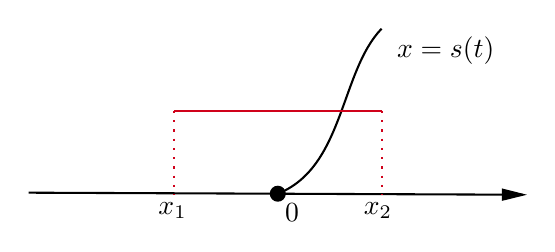
\begin{tikzpicture}[x=0.75pt,y=0.75pt,yscale=-1,xscale=1]
        %uncomment if require: \path (0,129); %set diagram left start at 0, and has height of 129

        %Straight Lines [id:da5683627584715716] 
        \draw    (180,89) -- (418,89.99) ;
        \draw [shift={(420,90)}, rotate = 180.24] [fill={rgb, 255:red, 0; green, 0; blue, 0 }  ][line width=0.08]  [draw opacity=0] (12,-3) -- (0,0) -- (12,3) -- cycle    ;
        %Curve Lines [id:da011225527952760883] 
        \draw    (300,89.5) .. controls (332,76.78) and (330,30.78) .. (350,10) ;
        \draw [shift={(300,89.5)}, rotate = 338.32] [color={rgb, 255:red, 0; green, 0; blue, 0 }  ][fill={rgb, 255:red, 0; green, 0; blue, 0 }  ][line width=0.75]      (0, 0) circle [x radius= 3.35, y radius= 3.35]   ;
        %Straight Lines [id:da9226910467281164] 
        \draw [color={rgb, 255:red, 208; green, 2; blue, 27 }  ,draw opacity=1 ]   (250,49.5) -- (350,49.5) ;
        %Straight Lines [id:da14727582197982603] 
        \draw [color={rgb, 255:red, 208; green, 2; blue, 27 }  ,draw opacity=1 ] [dash pattern={on 0.84pt off 2.51pt}]  (350,49.5) -- (350,90) ;
        %Straight Lines [id:da42108546755319476] 
        \draw [color={rgb, 255:red, 208; green, 2; blue, 27 }  ,draw opacity=1 ] [dash pattern={on 0.84pt off 2.51pt}]  (250,49.5) -- (250,90) ;

        % Text Node
        \draw (241,92.4) node [anchor=north west][inner sep=0.75pt]    {$x_{1}$};
        % Text Node
        \draw (340,92.4) node [anchor=north west][inner sep=0.75pt]    {$x_{2}$};
        % Text Node
        \draw (302,92.9) node [anchor=north west][inner sep=0.75pt]    {$0$};
        % Text Node
        \draw (356,12.4) node [anchor=north west][inner sep=0.75pt]    {$x=s(t)$};

    \end{tikzpicture}

\end{figure}
\FloatBarrier

\begin{align*}
    \frac{\de}{\dt}\int ^{x_{2}}_{x_{1}} \rho (y,t) \dy & =\frac{\de}{\dt}\left(\int ^{s(t)}_{x_{1}} +\int ^{x_{2}}_{s(t)}\right)                                                                                             \\
                                                        & =\int ^{s(t)}_{x_{1}} \rho _{t}(y,t) \dy\textcolor[rgb]{0.82,0.01,0.11}{+} \rho \left(s(t)\textcolor[rgb]{0.82,0.01,0.11}{^{-}} ,t\right) \cdotp \dot{s}(t)         \\
                                                        & \ \ \ \ +\int ^{x_{2}}_{s(t)} \rho _{t}(y,t) \dy\textcolor[rgb]{0.82,0.01,0.11}{-} \rho \left(s(t)\textcolor[rgb]{0.82,0.01,0.11}{^{+}} ,t\right) \cdotp \dot{s}(t)
\end{align*}
Riaccorpando l'integrale e sostituendo
\begin{equation*}
    \int ^{x_{2}}_{x_{1}} \rho _{t}(y,t) \dy+\left[ \rho \left(s(t)\textcolor[rgb]{0.82,0.01,0.11}{^{-}} ,t\right) -\rho \left(s(t)\textcolor[rgb]{0.82,0.01,0.11}{^{+}} ,t\right)\right] \cdotp \dot{s}(t) =q(\rho (x_{1} ,t)) -q(\rho (x_{2} ,t))
\end{equation*}
facendo il limite per $x_{2}\rightarrow s(t)^{+} ,x_{1}\rightarrow s(t)^{-}$
\begin{equation*}
    \underbrace{\int ^{x_{2}}_{x_{1}} \rho _{t}(y,t) \dy}_{\rightarrow 0} +\left[ \rho \left(s(t)\textcolor[rgb]{0.82,0.01,0.11}{^{-}} ,t\right) -\rho \left(s(t)\textcolor[rgb]{0.82,0.01,0.11}{^{+}} ,t\right)\right] \cdotp \dot{s}(t) =q\left(\rho \left(s(t)^{-} ,t\right)\right) -q\left(\rho \left(s(t)^{+} ,t\right)\right)
\end{equation*}
allora
\begin{equation}
    \dot{s}(t) =\frac{q\left(\rho \left(s(t)^{-} ,t\right)\right) -q\left(\rho \left(s(t)^{+} ,t\right)\right)}{\rho \left(s(t)^{-} ,t\right) -\rho \left(s(t)^{+} ,t\right)} =\frac{[ q(\rho)]^{+}_{-}}{[ \rho ]^{+}_{-}}
\end{equation}
Questa si chiama \textbf{condizione di Rankine-Hugoniot}, e rappresenta la legge di conservazione per la linea di discontinuità.

Nel caso del traffico\footnote{ricordiamo che era $q(\rho) =v_{m}\left(\rho -\frac{\rho ^{2}}{\rho _{m}}\right)$}
\begin{equation*}
    \rho ^{+} =\rho _{m} \ \ \ \ \rho ^{-} =\frac{1}{8} \rho _{m} \ \ \ \ \ \ \ \ q\left(\rho ^{+}\right) =0\ \ \ \ q\left(\rho ^{-}\right) =v_{m}\left(\frac{1}{8} \rho _{m} -\frac{1}{64} \rho _{m}\right) =\frac{7}{64} v_{m} \rho _{m}
\end{equation*}
quindi
\begin{equation*}
    \dot{s}(t) =\frac{q\left(\rho ^{-}\right) -q\left(\rho ^{+}\right)}{\rho ^{-} -\rho ^{+}} =\frac{\frac{7}{64} v_{m} \rho _{m} -0}{\frac{1}{8} \rho _{m} -\rho _{m}} =-\frac{1}{8} v_{m}
\end{equation*}
Siccome $s(0) =0$ la linea d'urto è data da
\begin{equation*}
    s(t) =-\frac{1}{8} v_{m} \cdotp t
\end{equation*}

\fg{0.7}{leggi-conservazione-trafico-urto}

\begin{equation*}
    \rho (x,t) =
    \begin{cases}
        \frac{1}{8} \rho _{m} & x< -\frac{1}{8} v_{m} t \\
        \rho _{m}             & x >-\frac{1}{8} v_{m} t
    \end{cases}
\end{equation*}
La linea d'urto rappresenta \textit{l'ingorgo} che si propaga all'indietro.
\fg[Soluzione del traffico a valle.]{0.6}{fig-soluzione-traffico-valle}

\LezioneS{25/03/2021}
\section{Ritorno al metodo delle caratteristiche}

Riprendiamo la soluzione dell'onda progressiva con velocità locale ottenuta dal metodo delle caratteristiche. Dato il problema di Cauchy
\begin{equation*}
    \begin{cases}
        u_{t} +q(u)_{x} =0 & x\in \mathbb{R} ,\ t >0 \\
        u(x,0) =g(x)       & x\in \mathbb{R}
    \end{cases}
\end{equation*}
la soluzione
\begin{align*}
    u(x,t) =g[ x-q'(g(\xi)) t] & \ \ \text{con} \ q'(g(\xi)) \ \text{velocità locale} \\
    \ x=q'(g(\xi)) t+\xi       & \ \ \text{caratteristica uscente da} \ \xi
\end{align*}
non è sempre valida. Nel caso del traffico ad esempio $q$ è concava
\begin{equation*}
    q(u) =\left(u-\frac{u^{2}}{\rho _{m}}\right) v_{m}
\end{equation*}

\begin{figure}[htpb]
    \centering
    \tikzset{every picture/.style={line width=0.75pt}} %set default line width to 0.75pt        

    \begin{tikzpicture}[x=0.75pt,y=0.75pt,yscale=-1,xscale=1]
        %uncomment if require: \path (0,136); %set diagram left start at 0, and has height of 136

        %Straight Lines [id:da2875962130576233] 
        \draw    (80,100) -- (383,100) ;
        \draw [shift={(385,100)}, rotate = 180] [fill={rgb, 255:red, 0; green, 0; blue, 0 }  ][line width=0.08]  [draw opacity=0] (12,-3) -- (0,0) -- (12,3) -- cycle    ;
        %Shape: Parabola [id:dp055144157028466756] 
        \draw   (262,100) .. controls (222.33,11.33) and (182.67,11.33) .. (143,100) ;

        % Text Node
        \draw (137,106.4) node [anchor=north west][inner sep=0.75pt]    {$0$};
        % Text Node
        \draw (240,106.4) node [anchor=north west][inner sep=0.75pt]    {$\rho _{m}$};
        % Text Node
        \draw (293,34.4) node [anchor=north west][inner sep=0.75pt]    {$q''< 0$};
        % Text Node
        \draw (358,105.4) node [anchor=north west][inner sep=0.75pt]    {$u$};

    \end{tikzpicture}
\end{figure}
\FloatBarrier

E abbiamo esaminato due casi
\begin{enumerate}
    \item Onda di rarefazione (dato decresente): ``$\displaystyle g'< 0$''\footnote{uso le virgolette perché nel senso delle distribuzioni.}

          \begin{figure}[htpb]
              \centering
              \tikzset{every picture/.style={line width=0.75pt}} %set default line width to 0.75pt        

              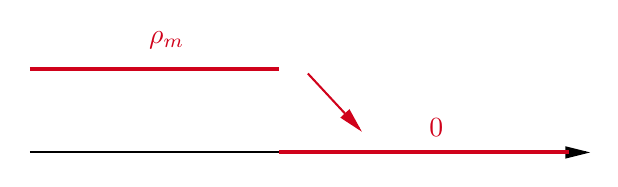
\begin{tikzpicture}[x=0.75pt,y=0.75pt,yscale=-1,xscale=1]
                  %uncomment if require: \path (0,94); %set diagram left start at 0, and has height of 94

                  %Straight Lines [id:da6720220897249527] 
                  \draw    (70,70) -- (338,70) ;
                  \draw [shift={(340,70)}, rotate = 180] [fill={rgb, 255:red, 0; green, 0; blue, 0 }  ][line width=0.08]  [draw opacity=0] (12,-3) -- (0,0) -- (12,3) -- cycle    ;
                  %Straight Lines [id:da05963541340200984] 
                  \draw [color={rgb, 255:red, 208; green, 2; blue, 27 }  ,draw opacity=1 ][line width=1.5]    (70,30) -- (190,30) ;
                  %Straight Lines [id:da8736597487715458] 
                  \draw [color={rgb, 255:red, 208; green, 2; blue, 27 }  ,draw opacity=1 ][line width=1.5]    (190,70) -- (330,70) ;
                  %Straight Lines [id:da04569768747860148] 
                  \draw [color={rgb, 255:red, 208; green, 2; blue, 27 }  ,draw opacity=1 ]   (204,32) -- (208.87,37.24) -- (228.64,58.53) ;
                  \draw [shift={(230,60)}, rotate = 227.12] [fill={rgb, 255:red, 208; green, 2; blue, 27 }  ,fill opacity=1 ][line width=0.08]  [draw opacity=0] (12,-3) -- (0,0) -- (12,3) -- cycle    ;

                  % Text Node
                  \draw (126,10.4) node [anchor=north west][inner sep=0.75pt]  [color={rgb, 255:red, 208; green, 2; blue, 27 }  ,opacity=1 ]  {$\rho _{m}$};
                  % Text Node
                  \draw (261,52.4) node [anchor=north west][inner sep=0.75pt]  [color={rgb, 255:red, 208; green, 2; blue, 27 }  ,opacity=1 ]  {$0$};

              \end{tikzpicture}
          \end{figure}
          \FloatBarrier

    \item Onda d'urto (dato crescente): ``$\displaystyle g' >0$''

          \begin{figure}[htpb]
              \centering
              \tikzset{every picture/.style={line width=0.75pt}} %set default line width to 0.75pt        

              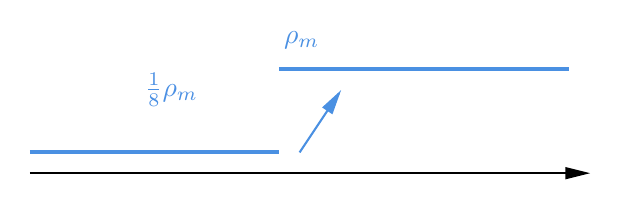
\begin{tikzpicture}[x=0.75pt,y=0.75pt,yscale=-1,xscale=1]
                  %uncomment if require: \path (0,94); %set diagram left start at 0, and has height of 94

                  %Straight Lines [id:da7883917441648187] 
                  \draw    (70,70) -- (338,70) ;
                  \draw [shift={(340,70)}, rotate = 180] [fill={rgb, 255:red, 0; green, 0; blue, 0 }  ][line width=0.08]  [draw opacity=0] (12,-3) -- (0,0) -- (12,3) -- cycle    ;
                  %Straight Lines [id:da35316348300621603] 
                  \draw [color={rgb, 255:red, 74; green, 144; blue, 226 }  ,draw opacity=1 ][line width=1.5]    (70,60) -- (190,60) ;
                  %Straight Lines [id:da1507199654174245] 
                  \draw [color={rgb, 255:red, 74; green, 144; blue, 226 }  ,draw opacity=1 ][line width=1.5]    (190,20) -- (330,20) ;
                  %Straight Lines [id:da08675484861458749] 
                  \draw [color={rgb, 255:red, 74; green, 144; blue, 226 }  ,draw opacity=1 ]   (200,60) -- (218.89,31.66) ;
                  \draw [shift={(220,30)}, rotate = 483.69] [fill={rgb, 255:red, 74; green, 144; blue, 226 }  ,fill opacity=1 ][line width=0.08]  [draw opacity=0] (12,-3) -- (0,0) -- (12,3) -- cycle    ;

                  % Text Node
                  \draw (124,20.4) node [anchor=north west][inner sep=0.75pt]  [color={rgb, 255:red, 208; green, 2; blue, 27 }  ,opacity=1 ]  {$\textcolor[rgb]{0.29,0.56,0.89}{\frac{1}{8}}\textcolor[rgb]{0.29,0.56,0.89}{\rho }\textcolor[rgb]{0.29,0.56,0.89}{_{m}}$};
                  % Text Node
                  \draw (191,0.4) node [anchor=north west][inner sep=0.75pt]  [color={rgb, 255:red, 74; green, 144; blue, 226 }  ,opacity=1 ]  {$\rho _{m}$};

              \end{tikzpicture}
          \end{figure}
          \FloatBarrier

          La linea di shock è determinabile tramite la relazione di Rankine-Hugoniot.
\end{enumerate}

Notiamo che se $g'$ è concorde con $q''$ abbiamo un'onda di rarefazione, se sono discordi un'onda d'urto. Cerchiamo di generalizzare questa affermazione.

Prendiamo la soluzione
\begin{equation*}
    u(x,t) =g(x-q'(g(\xi)) t)
\end{equation*}
Sulla caratteristica
\begin{equation*}
    x=q'(g(\xi))t +\xi
\end{equation*}
abbiamo che
\begin{equation*}
    u=g(\xi)
\end{equation*}
perché il dato che trasporta la caratteristica è proprio $\displaystyle g(\xi)$. Quindi posso riscrivere
\begin{equation*}
    u(x,t) =g(x-q'(g(\xi)) t) =g(x-q'(u) t)
\end{equation*}
Se prendo la funzione
\begin{equation*}
    G(x,t,u) =u-g(x-q'(u) t) =0
\end{equation*}
e la pongo uguale a $0$ ottengo un'equazione che, nel caso in cui il metodo delle caratteristiche funziona, definisce \textbf{implicitamente} $\displaystyle u=u(x,t)$.

\begin{theorem}
    [Teorema del Dini] Sia $A\subset \mathbb{R}^2$ aperto, $g:A\to \mathbb{R} $ una funzione $C^{1}(A) $. Consideriamo un punto $(x_{0},y_{0})\in A$ e supponiamo che $g(x_{0},y_{0})=0$ e che $g_{y}(x_{0},y_{0})\neq 0$. Allora esistono due intervalli reali $I,J$ tali da contenere $x_{0},y_{0}$ ed esiste unica una funzione $y(x):I\to J, y\in C^{1}(I) $ tale che $y(x_{0})=y_{0}$ e che $y'(x_{0})=-\frac{g_{x}(x_{0},y_{0})}{g_{y}(x_{0},y_{0})}$ e che per ogni $x,y$ nei due intervalli $I,J$ risulti che $g(x,y)=0 \Leftrightarrow y=y(x)$
\end{theorem}

Ma quando va ``tutto bene''?

Possiamo rispondere a questa domanda col \textbf{teorema di Dini}: $u$ è definita e regolare come funzione di $(x,t)$ se $g$ e $q'$ sono regolari e
\begin{equation*}
    G_{u}(x,t,u) =1+g'(\underbrace{x-q'(u) t}_{\xi }) q''(u) t\neq 0
\end{equation*}
possiamo riscrivere la condizione essendo $\displaystyle u=g(\xi)$ lungo la caratteristica:
\begin{equation}
    \boxed{G_{u} =1+g'(\xi) q''(g(\xi)) t\neq 0}
\end{equation}
\begin{itemize}
    \item La condizione sarà \textbf{sempre} soddisfatta se
          \begin{equation*}
              g'(\xi) q''(g(\xi)) \geq 0\ \text{in} \ \mathbb{R}
              \label{eq:condizione-tutto-bene}
          \end{equation*}
    \item Avrò problemi (\textbf{da un certo tempo in poi}) se
          \begin{equation*}
              g'(\xi) q''(g(\xi)) < 0
          \end{equation*}
\end{itemize}
\begin{nb}
    La pendenza della caratteristica è $\displaystyle q'(g(\xi)) .$ La condizione \eqref{eq:condizione-tutto-bene} equivale a:
    \begin{equation*}
        \frac{\de}{\dxi } q'(g(\xi)) =g'(\xi) q''(g(\xi)) \geq 0
    \end{equation*}
    ovvero richiediamo che le pendenze delle caratteristiche siano crescenti con $\xi $: le caratteristiche non si incontrano mai (se la derivata della pendenza è $0$, rimangono parallele, se è $< 0$ si intersecheranno dando origine ad una linea di shock).

    In figura si vede prima un caso di pendenza in aumento, quindi di condizione verificata (onda di rarefazione), poi un caso di pendenza che diminuisce (shock).

    \begin{figure}[H]
        \centering
        \tikzset{every picture/.style={line width=0.75pt}} %set default line width to 0.75pt        

        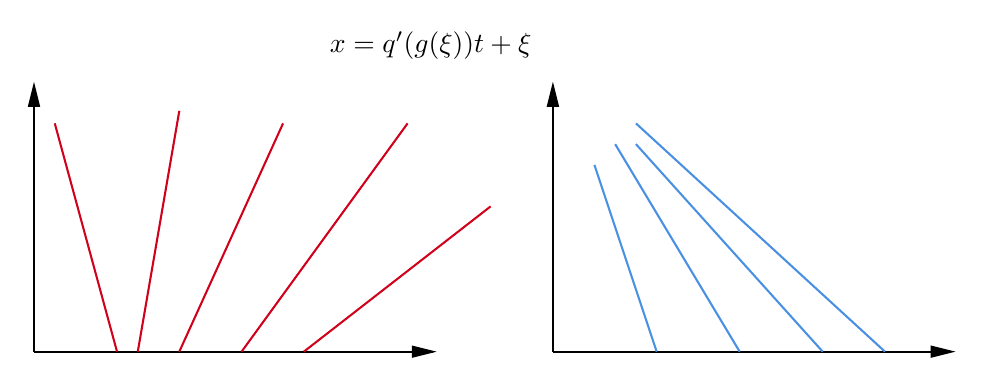
\begin{tikzpicture}[x=0.75pt,y=0.75pt,yscale=-1,xscale=1]
            %uncomment if require: \path (0,186); %set diagram left start at 0, and has height of 186

            %Straight Lines [id:da18552922863082344] 
            \draw    (50,160) -- (242,160) ;
            \draw [shift={(244,160)}, rotate = 180] [fill={rgb, 255:red, 0; green, 0; blue, 0 }  ][line width=0.08]  [draw opacity=0] (12,-3) -- (0,0) -- (12,3) -- cycle    ;
            %Straight Lines [id:da6920953070372635] 
            \draw    (300,160) -- (492,160) ;
            \draw [shift={(494,160)}, rotate = 180] [fill={rgb, 255:red, 0; green, 0; blue, 0 }  ][line width=0.08]  [draw opacity=0] (12,-3) -- (0,0) -- (12,3) -- cycle    ;
            %Straight Lines [id:da9506355610004393] 
            \draw    (50,160) -- (50,32) ;
            \draw [shift={(50,30)}, rotate = 450] [fill={rgb, 255:red, 0; green, 0; blue, 0 }  ][line width=0.08]  [draw opacity=0] (12,-3) -- (0,0) -- (12,3) -- cycle    ;
            %Straight Lines [id:da7876098730580057] 
            \draw    (300,160) -- (300,32) ;
            \draw [shift={(300,30)}, rotate = 450] [fill={rgb, 255:red, 0; green, 0; blue, 0 }  ][line width=0.08]  [draw opacity=0] (12,-3) -- (0,0) -- (12,3) -- cycle    ;
            %Straight Lines [id:da057799582697692475] 
            \draw [color={rgb, 255:red, 208; green, 2; blue, 27 }  ,draw opacity=1 ]   (60,50) -- (90,160) ;
            %Straight Lines [id:da5101748898124889] 
            \draw [color={rgb, 255:red, 208; green, 2; blue, 27 }  ,draw opacity=1 ]   (120,44) -- (100,160) ;
            %Straight Lines [id:da8896303791051883] 
            \draw [color={rgb, 255:red, 208; green, 2; blue, 27 }  ,draw opacity=1 ]   (170,50) -- (120,160) ;
            %Straight Lines [id:da9600961733527333] 
            \draw [color={rgb, 255:red, 208; green, 2; blue, 27 }  ,draw opacity=1 ]   (230,50) -- (150,160) ;
            %Straight Lines [id:da8447998484472494] 
            \draw [color={rgb, 255:red, 208; green, 2; blue, 27 }  ,draw opacity=1 ]   (270,90) -- (180,160) ;
            %Straight Lines [id:da5447595063496167] 
            \draw [color={rgb, 255:red, 74; green, 144; blue, 226 }  ,draw opacity=1 ]   (340,50) -- (460,160) ;
            %Straight Lines [id:da8739539798936098] 
            \draw [color={rgb, 255:red, 74; green, 144; blue, 226 }  ,draw opacity=1 ]   (340,60) -- (430,160) ;
            %Straight Lines [id:da7420335528346504] 
            \draw [color={rgb, 255:red, 74; green, 144; blue, 226 }  ,draw opacity=1 ]   (330,60) -- (390,160) ;
            %Straight Lines [id:da9739933109291887] 
            \draw [color={rgb, 255:red, 74; green, 144; blue, 226 }  ,draw opacity=1 ]   (320,70) -- (350,160) ;

            % Text Node
            \draw (191,4.4) node [anchor=north west][inner sep=0.75pt]    {$x=q'(g(\xi)) t+\xi $};

        \end{tikzpicture}
    \end{figure}
    \FloatBarrier
\end{nb}
Formalizziamo in un teorema.
\begin{theorem}
    Sia $\displaystyle q\in C^{2}(\mathbb{R}) ,\ g\in C^{1}(\mathbb{R})$ e $\displaystyle g'(\xi) q''(g(\xi)) \geq 0\ \forall \xi \in \mathbb{R}$. Allora l'equazione
    \begin{equation*}
        G(x,t,u) =u-g(x-q'(u) t) =0
    \end{equation*}
    definisce univocamente (\textbf{esistenza e unicità}) $\displaystyle u=u(x,t) \in C^{1}(\mathbb{R} \times [ 0,+\infty))$.
\end{theorem}
Qui abbiamo sia esistenza che unicità. Sebbene per il traffico abbiamo trovato delle soluzioni, non possiamo stabilire se sono uniche, perché i dati non sono regolari, in particolare $g$ non era $C^{1} $, era discontinua. Vedremo che l'unicità non è garantita, a meno di cercare particolari soluzioni, dette \emph{entropiche}, che saranno uniche sotto certe ipotesi.
\begin{dimostrazione}
    $u$ è definita univocamente per il teorema del Dini. Dimostriamo che $\displaystyle u\in C^{1}$. Sempre usando il teorema del Dini
    \begin{gather*}
        u_{t} =-\frac{G_{t}(x,t,u)}{G_{u}(x,t,u)} =-\frac{g'(x-q'(u) t) q'(u)}{1+\underbrace{tq''(u) g'(x-q'(u) t}_{\geq 0})}\\
        u_{x} =-\frac{G_{x}(x,t,u)}{G_{u}(x,t,u)} =\frac{g'(x-q'(u) t)}{1+\underbrace{tq''(u) g'(x-q'(u) t}_{\geq 0})}
    \end{gather*}
    allora
    \begin{equation*}
        u_{t} ,\ u_{x} \in C(\mathbb{R} \times [ 0,+\infty))
    \end{equation*}
    essendo continue (il denominatore non si annulla) perché rapporti di funzioni continue.
\end{dimostrazione}
Se invece
\begin{equation*}
    g'(\xi) q''(g(\xi)) < 0\ \text{in} \ [ a,b]
\end{equation*}
\begin{equation*}
    G_{u} =1+\underbrace{g'(\xi) q''(g(\xi))}_{< 0} t
\end{equation*}
ci aspettiamo l'\textbf{intersezione} delle caratteristiche e la formazione di uno shock. Ci poniamo il problema di determinare l'istante $\displaystyle t_{s}$ (breaking time) e il punto $\displaystyle x_{s}$ in cui parte la linea d'urto.
\begin{equation*}
    G_{u} =0 \quad \text{se}  \quad t(\xi) =\frac{1}{\underbrace{-g'(\xi) q''(g(\xi))}_{=z(\xi)}}
\end{equation*}
Per ogni $\xi $ trovo un tempo in cui $\displaystyle G_{u} =0$. Ma allora $\displaystyle t_{s}$ sarà il più piccolo tra questi tempi $\displaystyle t(\xi)$: assumiamo che in $\displaystyle [ a,b]$ $z$ abbia un solo punto di massimo $\displaystyle \xi _{M}$, allora il tempo di prima formazione dello shock sarà
\begin{equation*}
    t_{s} = \min_{\xi \in [a,b]}\frac{1}{z(\xi)}= \frac{1}{z(\xi _{M})}
\end{equation*}
$\displaystyle x_{s}$ si trova lungo la caratteristica che esce da $\displaystyle \xi _{M}$ al tempo $\displaystyle t_{s}$
\begin{equation*}
    x_{s} =q'(g(\xi _{M})) t_{s} +\xi _{M} =q'(g(\xi _{M}))\frac{1}{z(\xi _{M})} +\xi _{M}
\end{equation*}
Il punto $(x_{s},t_{s})$ ha un interessante significato geometrico, esaminiamo il seguente esempio.
\textbf{Esempio.}
\begin{equation*}
    \begin{cases}
        u_{t} +(1-2u) u_{x} =0 \\
        u(x,0) =\arctan x
    \end{cases}
\end{equation*}
\begin{align*}
    q(u)   & =u-u^{2} & g(\xi)  & =\arctan \xi          \\
    q'(u)  & =1-2u    & g'(\xi) & =\frac{1}{1+\xi ^{2}} \\
    q''(u) & =-2      &         &
\end{align*}
Abbiamo $\displaystyle g' >0,q''< 0$ discordi, ci aspettiamo uno shock.
\begin{equation*}
    z(\xi) = - \underbrace{g'(\xi)}_{\frac{1}{1+\xi^2}} \underbrace{q''(g(\xi))}_{-2} =\frac{2}{1+\xi ^{2}} \Rightarrow \ \xi _{M} =0
\end{equation*}
Allora $\displaystyle z(\xi _{M}) =2$ e lo shock parte da
\begin{equation*}
    t_{s} =\frac{1}{z(\xi _{M})} =\frac{1}{2} ,\quad x_{s} =q'(g(\xi _{M}))\frac{1}{2} +0=q'(0)\frac{1}{2} =\frac{1}{2}
\end{equation*}
Geometricamente, $u$ è definita da
\begin{equation*}
    G(x,t,u) = u-g(x-q'(u)t)= u-\arctan(x-(1-2u) t) =0,\ \text{per} \ t< \frac{1}{2}
\end{equation*}

\fg[Breaking time per il problema]{0.6}{leggi-conservazione-esempio-bt}

Dopo $\displaystyle t_{s}$ la linea di livello di $G$ non definisce più il grafico di una funzione.
\fg[Plot del problema]{0.6}{fig-breaking-time}
Si può dimostrare però che se tracciamo una retta verticale (tagliando due aree $A$ e $B$ di ugual area) otteniamo $\displaystyle s(t)$ dato dalle condizioni di Rankine-Hugoniot.

\fg[Inserimento di uno shock con la regola di Whitham.]{0.6}{leggi-conservazione-esempio-taglio}

\LezioneS{29/03/2021}
\section{Soluzione debole}

Abbiamo notato una serie di problemi nel determinare la soluzione di \eqref{eq:conservazione-formulazione-forte} nel caso in cui $g$ avesse una qualche discontinuità
\begin{equation}
    \tag{P$_{\text{cons,forte}}$}
    \begin{cases}
        u_{t} +q(u)_{x} =0 & x\in \mathbb{R} ,\ t >0 \\
        u(x,0) =g(x)       & x\in \mathbb{R}
    \end{cases}
    \label{eq:conservazione-formulazione-forte}
\end{equation}
\begin{enumerate}
    \item Dobbiamo dare \textbf{senso} al concetto di soluzione quando si presentano discontinuità (\textit{onde di rarefazione, onde d'urto o shock}).
    \item Abbiamo costruito, nel caso di rarefazione, una soluzione con approssimazioni. Questo tuttavia non garantisce \textbf{unicità}. Se siamo in presenza di più soluzioni dobbiamo fornire un criterio di \textit{selezione} che possa individuare (preferibilmente) un'unica soluzione che ha \textbf{senso fisico}.
\end{enumerate}

Allarghiamo il concetto di soluzione introducendo la \textbf{soluzione debole} (o \textbf{soluzione integrale}, o \textbf{soluzione generalizzata}).
\begin{definition}
    [Soluzione classica o regolare] $u\in C^{1}(\mathbb{R} \times \textcolor[rgb]{0.82,0.01,0.11}{[} 0,+\infty))$.
\end{definition}
\begin{definition}
    [Funzione test] $v\in C^{1}(\mathbb{R} \times [ 0,+\infty))$ a supporto compatto.
\end{definition}
Sia $u$ soluzione classica, $v$ funzione test, moltiplichiamo \eqref{eq:conservazione-formulazione-forte} con la funzione test e integriamo
\begin{equation*}
    \underbrace{\int ^{+\infty }_{0}\int _{\mathbb{R}} vu_{t} \dx\dt}_{A} +\underbrace{\int ^{+\infty }_{0}\int _{\mathbb{R}} vq(u)_{x} \dx\dt}_{B} =0
\end{equation*}
Integriamo $A$ per parti rispetto a $t$ e usiamo il supporto compatto
\begin{align*}
    A & =\int _{\mathbb{R}}[ vu]^{+\infty }_{0} \dx-\int ^{+\infty }_{0}\int _{\mathbb{R}} uv_{t} \dx\dt                                                                        \\
      & = \cancel{\int _{\mathbb{R}} v(x,\infty) u(x,\infty) \dx} -\int _{\mathbb{R}} v(x,0)\underbrace{u(x,0)}_{g(x)} \dx-\int ^{+\infty }_{0}\int _{\mathbb{R}} uv_{t} \dx\dt \\
      & =-\int _{\mathbb{R}} v(x,0) g(x) \dx-\int ^{+\infty }_{0}\int _{\mathbb{R}} uv_{t} \dx\dt
\end{align*}
Integriamo $B$ per parti rispetto a $x$
\begin{align*}
    B & =\cancel{\int ^{+\infty }_{0}[ vq(u)]^{+\infty }_{-\infty } dt} -\int ^{+\infty }_{0}\int _{\mathbb{R}} v_{x} q(u) \dx\dt
\end{align*}
Segue che
\begin{equation}
    \tag{P$_{\text{cons,debole}}$}
    \int ^{+\infty }_{0}\int _{\mathbb{R}}[ uv_{t} +q(u) v_{x}] \dx\dt+\int _{\mathbb{R}} v(x,0) g(x) \dx=0\ \ \forall \ v
    \label{eq:conservazione-formulazione-debole}
\end{equation}
che chiameremo \textbf{formulazione debole}. Notiamo che \textit{non compaiono le derivate di} $u$. Quindi
\begin{equation*}
    u\ \text{regolare} \ \ \Rightarrow \ \ \text{implica la formulazione debole}
\end{equation*}
Possiamo tornare indietro? Sì.

Partendo dalla formulazione debole \eqref{eq:conservazione-formulazione-debole} e integrando per parti in senso inverso il primo termine, stavolta coi ruoli delle funzioni invertiti rispetto al primo passaggio
\begin{equation}
    \int ^{+\infty }_{0}\int _{\mathbb{R}}[ u_{t}+q(u)_{x}] v\dx\dt\underbrace{+\int _{\mathbb{R}} v(x,0) u(x,0) \dx-\int _{\mathbb{R}} v(x,0) g(x) \dx}_{\int _{\mathbb{R}}[ u(x,0)-g(x)] v(x,0) \dx} =0
    \label{eq:formulazione-debole-passaggio-1}
\end{equation}
Che è valida per ogni funzione test, scelgo quindi $v$ test con supporto in $\mathbb{R} \times \textcolor[rgb]{0.82,0.01,0.11}{(} 0,+\infty)$, annullando tutto il secondo termine
\begin{equation*}
    \int ^{+\infty }_{0}\int _{\mathbb{R}}[ u_{t} +q(u)_{x}] v\dx\dt=0\ \ \forall \ \text{funzione test}
\end{equation*}
Per il lemma di annullamento ritroviamo la prima parte di \eqref{eq:conservazione-formulazione-forte}
\begin{equation*}
    u_{t} +q(u)_{x} =0
\end{equation*}
La inseriamo nella \eqref{eq:formulazione-debole-passaggio-1}
\begin{equation*}
    \int _{\mathbb{R}}[ g(x) -u(x,0)] v(x,0) =0\ \ \forall \ \text{funzione test}
\end{equation*}
Sempre per il lemma di annullamento ritroviamo la seconda parte (la condizione iniziale) di \eqref{eq:conservazione-formulazione-forte}
\begin{equation*}
    u(x,0) =g(x)
\end{equation*}
In conclusione
\begin{equation}
    u\ \text{regolare} \ \ \Leftrightarrow \ \ \text{implica la formulazione debole}
\end{equation}
\begin{theorem}
    [Lemma di annullamento] Sia $\Omega \subseteq \mathbb{R}^{n}$ aperto, sia $f\in C(\Omega)$ tale che
    \begin{equation}
        \int _{\Omega } fv\dxx=0, \quad \forall  v\in C^{1}(\Omega) \ \text{a supporto compatto}
    \end{equation}
    allora $f=0$ in $\Omega $.
\end{theorem}
\begin{dimostrazione}
    Se per assurdo $f(\x_{0}) \neq 0$, per esempio $f(\x_{0})  >0$, allora possiamo considerare $B_{r}(\x_{0}) \subset \Omega $ tale che $f(\x)>0$ in $B_{r}(\x_{0})$.

    \begin{figure}[H]
        \centering
        \tikzset{every picture/.style={line width=0.75pt}} %set default line width to 0.75pt        

        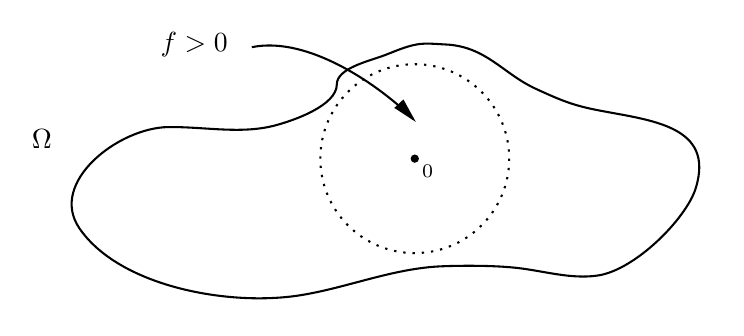
\begin{tikzpicture}[x=0.75pt,y=0.75pt,yscale=-1,xscale=1]
            %uncomment if require: \path (0,157); %set diagram left start at 0, and has height of 157

            %Shape: Free Drawing [id:dp3576446128815167] 
            \draw  [color={rgb, 255:red, 0; green, 0; blue, 0 }  ][line width=0.75] [line join = round][line cap = round] (289.46,42.15) .. controls (289.46,52.52) and (268.37,59.73) .. (259.5,62.05) .. controls (243.12,66.34) and (225.26,62.54) .. (208.15,62.79) .. controls (184.22,63.13) and (150.4,89.38) .. (165.35,111.44) .. controls (184.36,139.5) and (237.09,149.26) .. (271.49,143.87) .. controls (294.38,140.29) and (316.47,130.81) .. (339.96,129.87) .. controls (349.8,129.47) and (364.85,129.41) .. (375.91,130.61) .. controls (389.01,132.02) and (402.29,136.27) .. (415.29,134.29) .. controls (433.4,131.54) and (457.87,106.78) .. (462.36,92.27) .. controls (471.72,62.05) and (440.9,59.64) .. (415.29,54.68) .. controls (403.06,52.31) and (397.25,49.84) .. (385.33,44.36) .. controls (369.4,37.04) and (361.31,23.83) .. (341.67,22.98) .. controls (337.12,22.79) and (332.45,22.19) .. (327.98,22.98) .. controls (322.58,23.94) and (317.61,26.22) .. (312.57,28.14) .. controls (305.35,30.91) and (289.46,34.38) .. (289.46,42.15) -- cycle ;
            %Shape: Circle [id:dp058058363212611264] 
            \draw  [draw opacity=0][fill={rgb, 255:red, 0; green, 0; blue, 0 }  ,fill opacity=1 ] (325,78) .. controls (325,76.9) and (325.9,76) .. (327,76) .. controls (328.1,76) and (329,76.9) .. (329,78) .. controls (329,79.1) and (328.1,80) .. (327,80) .. controls (325.9,80) and (325,79.1) .. (325,78) -- cycle ;
            %Shape: Circle [id:dp45946265794375796] 
            \draw  [dash pattern={on 0.84pt off 2.51pt}] (281.5,78) .. controls (281.5,52.87) and (301.87,32.5) .. (327,32.5) .. controls (352.13,32.5) and (372.5,52.87) .. (372.5,78) .. controls (372.5,103.13) and (352.13,123.5) .. (327,123.5) .. controls (301.87,123.5) and (281.5,103.13) .. (281.5,78) -- cycle ;
            %Curve Lines [id:da9084321948695291] 
            \draw    (248.5,24.3) .. controls (276.63,18.48) and (312.29,44.65) .. (326.27,59) ;
            \draw [shift={(327.5,60.3)}, rotate = 227.12] [fill={rgb, 255:red, 0; green, 0; blue, 0 }  ][line width=0.08]  [draw opacity=0] (12,-3) -- (0,0) -- (12,3) -- cycle    ;

            % Text Node
            \draw (141,62.4) node [anchor=north west][inner sep=0.75pt]    {$\Omega $};
            % Text Node
            \draw (329,79.4) node [anchor=north west][inner sep=0.75pt]    {$\x_{0}$};
            % Text Node
            \draw (203,15.4) node [anchor=north west][inner sep=0.75pt]    {$f>0$};

        \end{tikzpicture}
    \end{figure}
    \FloatBarrier

    Possiamo allora sempre trovare una $v\in C^{1}(\Omega)$ tale che $v>0$ in $B_{r}(\x_{0})$ e $v=0$ in $\Omega \setminus \overline{B_{r}(\x_{0})}$ ma allora
    \begin{equation*}
        0 \overset{\text{hp}}{=} \int _{\Omega } fv\dxx=\int _{B_{r}(\x_{0})} fv\dxx >0
    \end{equation*}
    assurdo.
\end{dimostrazione}
\begin{definition}
    [Soluzione debole] Sia $u:\mathbb{R} \times [ 0,+\infty ]\rightarrow \mathbb{R}$ localmente limitata\footnote{cioè in ogni compatto.}. Diciamo che $u$ è \textbf{soluzione debole} del problema
    \begin{equation*}
        \begin{cases}
            u_{t} +q(u)_{x} =0 & x\in \mathbb{R} ,\ t >0 \\
            u(x,0) =g(x)       & x\in \mathbb{R}
        \end{cases}
    \end{equation*}
    se vale la \eqref{eq:conservazione-formulazione-debole}, cioè se
    \begin{equation*}
        \int ^{+\infty }_{0}\int _{\mathbb{R}}[ uv_{t} +q(u) v_{x}] \dx\dt+\int _{\mathbb{R}} v(x,0) g(x) \dx=0\ \ \forall \ \text{funzione test}
    \end{equation*}
\end{definition}
\subsection{Condizione di Rankine-Hugoniot}
\begin{theorem}
    Sia $u$ soluzione debole tale che
    \begin{enumerate}
        \item ha una linea di discontinuità a salto $x=s(t)$ di classe $C^{1}$
        \item fuori da $\Gamma $ è soluzione classica di $u_{t} +q(u)_{x} =0$
        \item il salto $\left[ u^{+} -u^{-}\right]_{|\Gamma }$ varia con continuità
    \end{enumerate}

    Allora
    \begin{equation}
        \dot{s}(t) =\frac{q\left(u^{+}\right) -q\left(u^{-}\right)}{u^{+} -u^{-}}
    \end{equation}
\end{theorem}
\begin{dimostrazione}
    Consideriamo un aperto $V$ contenuto nel semipiano $t >0$, diviso in due parti $V^{+} ,V^{-}$ da una linea $\Gamma $, definita da un'equazione $x=s(t)$, in cui $u(x,t)$ presenti una discontinuità di tipo salto, mentre al di fuori è soluzione classica.

    Consideriamo $v$ funzione test di supporto $K\subset V$, a cavallo di $\Gamma $.

    \begin{figure}[H]
        \centering
        \tikzset{every picture/.style={line width=0.75pt}} %set default line width to 0.75pt        

        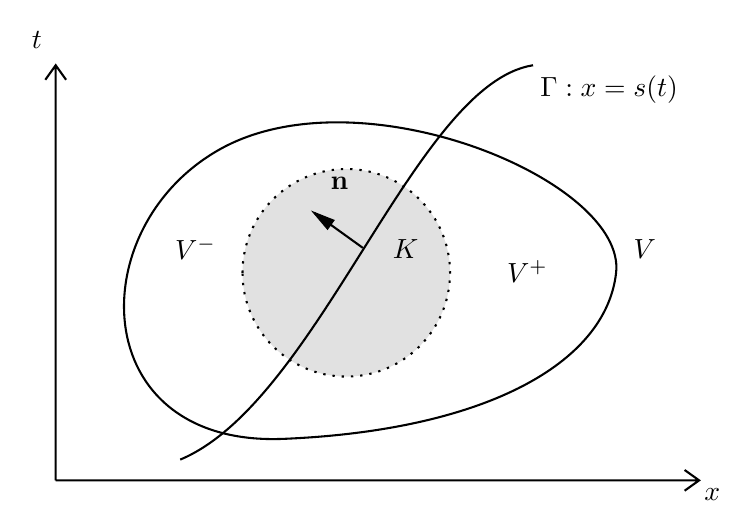
\begin{tikzpicture}[x=0.75pt,y=0.75pt,yscale=-1,xscale=1]
            %uncomment if require: \path (0,254); %set diagram left start at 0, and has height of 254

            %Shape: Circle [id:dp6540334045891043] 
            \draw  [fill={rgb, 255:red, 155; green, 155; blue, 155 }  ,fill opacity=0.3 ][dash pattern={on 0.84pt off 2.51pt}] (240,130) .. controls (240,102.39) and (262.39,80) .. (290,80) .. controls (317.61,80) and (340,102.39) .. (340,130) .. controls (340,157.61) and (317.61,180) .. (290,180) .. controls (262.39,180) and (240,157.61) .. (240,130) -- cycle ;
            %Shape: Axis 2D [id:dp8832982209867613] 
            \draw  (150,230) -- (460,230)(150,30) -- (150,230) -- cycle (453,225) -- (460,230) -- (453,235) (145,37) -- (150,30) -- (155,37)  ;
            %Shape: Polygon Curved [id:ds48614957603604325] 
            \draw   (230,70) .. controls (298,32.94) and (425,85.94) .. (420,130) .. controls (415,174.06) and (356,205.94) .. (260,210) .. controls (164,214.06) and (162,107.06) .. (230,70) -- cycle ;
            %Curve Lines [id:da07213479844491588] 
            \draw    (210,220) .. controls (277,191.94) and (323,38.94) .. (380,30) ;
            %Straight Lines [id:da7004760498060476] 
            \draw    (298,118) -- (274.62,101.17) ;
            \draw [shift={(273,100)}, rotate = 395.75] [fill={rgb, 255:red, 0; green, 0; blue, 0 }  ][line width=0.08]  [draw opacity=0] (12,-3) -- (0,0) -- (12,3) -- cycle    ;

            % Text Node
            \draw (461,232.4) node [anchor=north west][inner sep=0.75pt]    {$x$};
            % Text Node
            \draw (137,12.4) node [anchor=north west][inner sep=0.75pt]    {$t$};
            % Text Node
            \draw (366,122.4) node [anchor=north west][inner sep=0.75pt]    {$V^{+}$};
            % Text Node
            \draw (206,111.4) node [anchor=north west][inner sep=0.75pt]    {$V^{-}$};
            % Text Node
            \draw (382,33.4) node [anchor=north west][inner sep=0.75pt]    {$\Gamma :x=s(t)$};
            % Text Node
            \draw (427,112.4) node [anchor=north west][inner sep=0.75pt]    {$V$};
            % Text Node
            \draw (311,112.4) node [anchor=north west][inner sep=0.75pt]    {$K$};
            % Text Node
            \draw (281,82.4) node [anchor=north west][inner sep=0.75pt]    {$\mathbf{n}$};

        \end{tikzpicture}
    \end{figure}
    \FloatBarrier

    Essendo $V$ nel semipiano con $t >0$, e $K\subset V$, allora $v(x,t=0) =0$, allora la FD\footnote{Formulazione Debole.} diventa
    \begin{equation*}
        0=\int ^{+\infty }_{0}\int _{\mathbb{R}}[ uv_{t} +q(u) v_{x}] \dx\dt+\cancel{\int _{\mathbb{R}} v(x,0) g(x) \dx} =\int _{V} =\int _{V^{+}} +\int _{V^{-}}
    \end{equation*}
    Lavoriamo separatamente. Notiamo subito che possiamo scrivere la formula di derivata per parti
    \begin{align*}
        uv_{t}     & =(uv)_{t} -u_{t} v        \\
        q(u) v_{x} & =(q(u) v)_{x} -q(u)_{x} v
    \end{align*}
    che possiamo sostituire
    \begin{align*}
        0 & =\left(\int _{V^{+}} +\int _{V^{-}}\right)[ uv_{t} +q(u) v_{x}] \dx\dt                        \\
          & =\left(\int _{V^{+}} +\int _{V^{-}}\right)[(uv)_{t} +(q(u) v)_{x} -u_{t} v-q(u)_{x} v] \dx\dt
    \end{align*}
    sistemiamo i termini e raccogliamo $v$
    \begin{equation*}
        0=\left(\int _{V^{+}} +\int _{V^{-}}\right)[(uv)_{t} +(q(u) v)_{x}] \dx\dt-\left(\int _{V^{+}} +\int _{V^{-}}\right)[ u_{t} +q(u)_{x}] v\dx\dt
    \end{equation*}
    notiamo ora che $u$ al di fuori di $\Gamma $ è regolare e quindi soluzione classica\footnote{questo passaggio lo abbiamo potuto fare solo grazie al fatto che i due integrali sono separati su $V^{+} ,V^{-}$.} $u_{t} +q(u)_{x} =0$. Questo ci permette di cancellare il secondo termine
    \begin{equation*}
        0=\left(\int _{V^{+}} +\int _{V^{-}}\right)[(uv)_{t} +(q(u) v)_{x}] \dx\dt
    \end{equation*}
    Ciò che è in parentesi quadra altro non è che la divergenza di una funzione!
    \begin{gather*}
        \mathbf{v}(x,t) =
        \begin{pmatrix}
            q(u) v \\
            uv
        \end{pmatrix} \ \ \Rightarrow \ \ \mathrm{div} \ \mathbf{v} =(q(u) v)_{x} +(uv)_{t}\\
        \left(\int _{V^{+}} +\int _{V^{-}}\right)[(uv)_{t} +(q(u) v)_{x}] \dx\dt=\left(\int _{V^{+}} +\int _{V^{-}}\right)[\mathrm{div} \ \mathbf{v}] \dx\dt
    \end{gather*}
    pertanto possiamo applicare il Teorema della Divergenza. Consideriamo $\mathbf{n} =(n_{x} ,n_{t})$ normale, $n_{x}$ in $x$, $n_{t}$ in $t$, e ricordiamoci che
    \begin{itemize}
        \item la normale è entrante in $V^{-}$
        \item $v=0$ al di fuori di $K$
        \item quando scriviamo $u$ integrata su $\Gamma $ dobbiamo specificare se stiamo facendo il limite da destra o sinistra
    \end{itemize}
    \begin{align*}
        \int _{V^{+}}[\mathrm{div} \ \mathbf{v}] \dx\dt & =\int _{\partial V^{+}}\mathbf{v} \cdotp \mathbf{n} \dl=\left[\cancel{\int _{\partial V^{+} \setminus K}} +\int _{K\cap \Gamma }\right]
        \begin{pmatrix}
            q(u) v \\
            uv
        \end{pmatrix} \cdotp
        \begin{pmatrix}
            n_{x} \\
            n_{t}
        \end{pmatrix} \dl                                                                                                                                                              \\
                                                        & =\int _{K\cap \Gamma }\left[ q\left(u^{+}\right) n_{x} +u^{+} n_{t}\right] v\dl                                                            \\
                                                        &                                                                                                                                            \\
        \int _{V^{-}}[\mathrm{div} \ \mathbf{v}] \dx\dt & =\int _{\partial V^{-}}\mathbf{v} \cdotp (-\mathbf{n}) \dl=\left[\cancel{\int _{\partial V^{-} \setminus K}} +\int _{K\cap \Gamma }\right]
        \begin{pmatrix}
            q(u) v \\
            uv
        \end{pmatrix} \cdotp
        \begin{pmatrix}
            -n_{x} \\
            -n_{t}
        \end{pmatrix} \dl                                                                                                                                                              \\
                                                        & =\int _{K\cap \Gamma }\left[ -q\left(u^{-}\right) n_{x} -u^{-} n_{t}\right] v\dl
    \end{align*}
    A questo punto mettiamo insieme, possiamo tranquillamente portare tutto sotto lo stesso integrale
    \begin{equation*}
        0=\int _{K\cap \Gamma }\left[ q\left(u^{+}\right) n_{x} +u^{+} n_{t} -q\left(u^{-}\right) n_{x} -u^{-} n_{t}\right] v\dl\ \ \forall v
    \end{equation*}
    l'arbitrarietà di $v$ e il fatto che \emph{il salto varia con continuità}, fondamentale per usare il lemma di annullamento, ci fa concludere che
    \begin{equation*}
        q\left(u^{+}\right) n_{x} +u^{+} n_{t} -q\left(u^{-}\right) n_{x} -u^{-} n_{t} =0
    \end{equation*}
    A questo punto lo studente può rilassarsi, il peggio è passato, ci basta effettuare qualche passaggio algebrico per arrivare al risultato
    \begin{equation*}
        0=q\left(u^{+}\right) n_{x} +u^{+} n_{t} -q\left(u^{-}\right) n_{x} -u^{-} n_{t} =\left\{q\left(u^{+}\right) -q\left(u^{-}\right)\right\} n_{x} +\left\{u^{+} -u^{-}\right\} n_{t}
    \end{equation*}
    Ci dobbiamo solo ricordare che $\Gamma $ si può esprimere tramite $x=s(t)$ ed essendo $C^{1}$ il versore tangente alla curva è
    \begin{equation*}
        \mathbf{t} =\frac{1}{\sqrt{1+(\dot{s}(t))^{2}}}
        \begin{pmatrix}
            \dot{s}(t) \\
            1
        \end{pmatrix}
    \end{equation*}
    da cui si trova quello normale, sempre facendo riferimento alla figura
    \begin{equation*}
        \mathbf{n} =\frac{1}{\sqrt{1+(\dot{s}(t))^{2}}}
        \begin{pmatrix}
            -1 \\
            \dot{s}(t)
        \end{pmatrix}
    \end{equation*}
    Sostituiamo e moltiplichiamo tranquillamente per la radice, il cui unico e triste scopo era quello di avere dei versori
    \begin{align*}
        0 & =\left\{q\left(u^{+}\right) -q\left(u^{-}\right)\right\} n_{x} +\left\{u^{+} -u^{-}\right\} n_{t}     \\
          & =\left\{q\left(u^{+}\right) -q\left(u^{-}\right)\right\}(-1) +\left\{u^{+} -u^{-}\right\}(\dot{s}(t))
    \end{align*}
    Allora
    \begin{equation*}
        \dot{s}(t) =\frac{q\left(u^{+}\right) -q\left(u^{-}\right)}{u^{+} -u^{-}}
    \end{equation*}
    che è Rankine-Hugoniot.
\end{dimostrazione}

\textit{Controesempio all'unicità.}

Consideriamo l'equazione di Burgers
\begin{equation}
    u_{t} +uu_{x} =0\ \ \ \ q(u) =\frac{u^{2}}{2} ,\ \ q'(u) =u,\ \ q''(u) =1
\end{equation}
risolviamo il seguente problema di Cauchy
\begin{equation*}
    \begin{cases}
        u_{t} +uu_{x} =0 \\
        u(x,0) =g(x)
    \end{cases} \ \ \ \ g(x) =
    \begin{cases}
        0, & x< 0 \\
        1, & x >0
    \end{cases}
\end{equation*}
Secondo quanto detto prima, essendo $g'$ e $q''$ \emph{concordi} \textbf{non ci aspettiamo uno shock}.
le caratteristiche sono della forma
\begin{equation*}
    x=q'(g(x_{0})) t+x_{0} =
    \begin{cases}
        x_{0}   & x_{0} < 0 \\
        t+x_{0} & x_{0}  >0
    \end{cases}
\end{equation*}

\begin{figure}[H]
    \centering
    \tikzset{every picture/.style={line width=0.75pt}} %set default line width to 0.75pt        

    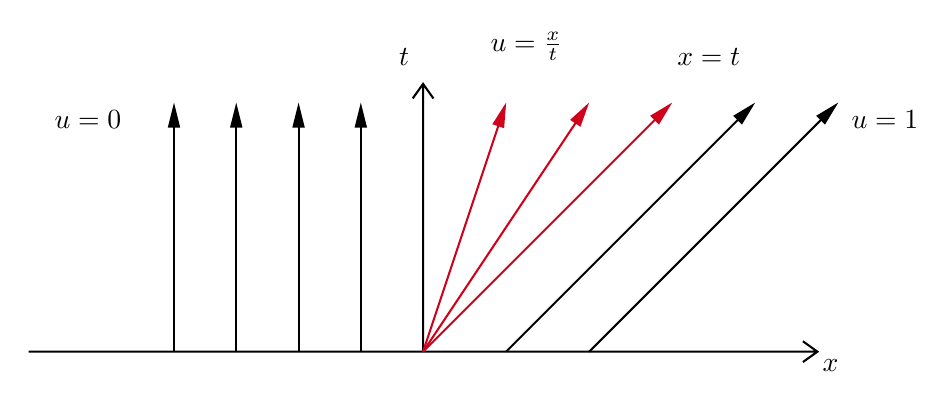
\begin{tikzpicture}[x=0.75pt,y=0.75pt,yscale=-1,xscale=1]
        %uncomment if require: \path (0,195); %set diagram left start at 0, and has height of 195

        %Shape: Axis 2D [id:dp8314331427479191] 
        \draw  (110,170) -- (490,170)(300,41) -- (300,170) (483,165) -- (490,170) -- (483,175) (295,48) -- (300,41) -- (305,48)  ;
        %Straight Lines [id:da8703316857521626] 
        \draw    (270,170) -- (270,52) ;
        \draw [shift={(270,50)}, rotate = 450] [fill={rgb, 255:red, 0; green, 0; blue, 0 }  ][line width=0.08]  [draw opacity=0] (12,-3) -- (0,0) -- (12,3) -- cycle    ;
        %Straight Lines [id:da23720350427828807] 
        \draw    (240,170) -- (240,52) ;
        \draw [shift={(240,50)}, rotate = 450] [fill={rgb, 255:red, 0; green, 0; blue, 0 }  ][line width=0.08]  [draw opacity=0] (12,-3) -- (0,0) -- (12,3) -- cycle    ;
        %Straight Lines [id:da6575869667008147] 
        \draw    (210,170) -- (210,52) ;
        \draw [shift={(210,50)}, rotate = 450] [fill={rgb, 255:red, 0; green, 0; blue, 0 }  ][line width=0.08]  [draw opacity=0] (12,-3) -- (0,0) -- (12,3) -- cycle    ;
        %Straight Lines [id:da36794993787678143] 
        \draw    (180,170) -- (180,52) ;
        \draw [shift={(180,50)}, rotate = 450] [fill={rgb, 255:red, 0; green, 0; blue, 0 }  ][line width=0.08]  [draw opacity=0] (12,-3) -- (0,0) -- (12,3) -- cycle    ;
        %Straight Lines [id:da10755395047947025] 
        \draw [color={rgb, 255:red, 208; green, 2; blue, 27 }  ,draw opacity=1 ]   (300,170) -- (418.59,51.41) ;
        \draw [shift={(420,50)}, rotate = 495] [fill={rgb, 255:red, 208; green, 2; blue, 27 }  ,fill opacity=1 ][line width=0.08]  [draw opacity=0] (12,-3) -- (0,0) -- (12,3) -- cycle    ;
        %Straight Lines [id:da572956781405489] 
        \draw    (340,170) -- (458.59,51.41) ;
        \draw [shift={(460,50)}, rotate = 495] [fill={rgb, 255:red, 0; green, 0; blue, 0 }  ][line width=0.08]  [draw opacity=0] (12,-3) -- (0,0) -- (12,3) -- cycle    ;
        %Straight Lines [id:da25434860970077944] 
        \draw    (380,170) -- (498.59,51.41) ;
        \draw [shift={(500,50)}, rotate = 495] [fill={rgb, 255:red, 0; green, 0; blue, 0 }  ][line width=0.08]  [draw opacity=0] (12,-3) -- (0,0) -- (12,3) -- cycle    ;
        %Straight Lines [id:da107304666557968] 
        \draw [color={rgb, 255:red, 208; green, 2; blue, 27 }  ,draw opacity=1 ]   (300,170) -- (378.89,51.66) ;
        \draw [shift={(380,50)}, rotate = 483.69] [fill={rgb, 255:red, 208; green, 2; blue, 27 }  ,fill opacity=1 ][line width=0.08]  [draw opacity=0] (12,-3) -- (0,0) -- (12,3) -- cycle    ;
        %Straight Lines [id:da9234903706480704] 
        \draw [color={rgb, 255:red, 208; green, 2; blue, 27 }  ,draw opacity=1 ]   (300,170) -- (339.37,51.9) ;
        \draw [shift={(340,50)}, rotate = 468.43] [fill={rgb, 255:red, 208; green, 2; blue, 27 }  ,fill opacity=1 ][line width=0.08]  [draw opacity=0] (12,-3) -- (0,0) -- (12,3) -- cycle    ;

        % Text Node
        \draw (121,52.4) node [anchor=north west][inner sep=0.75pt]    {$u=0$};
        % Text Node
        \draw (505,52.4) node [anchor=north west][inner sep=0.75pt]    {$u=1$};
        % Text Node
        \draw (491,172.4) node [anchor=north west][inner sep=0.75pt]    {$x$};
        % Text Node
        \draw (287,22.4) node [anchor=north west][inner sep=0.75pt]    {$t$};
        % Text Node
        \draw (421,22.4) node [anchor=north west][inner sep=0.75pt]    {$x=t$};
        % Text Node
        \draw (331,14.4) node [anchor=north west][inner sep=0.75pt]    {$u=\frac{x}{t}$};

    \end{tikzpicture}
\end{figure}
\FloatBarrier

inoltre $q'(u) =u$, allora $r(s)=s$ quindi
\begin{equation*}
    u(x,t) =r\left(\frac{x}{t}\right) =\frac{x}{t}
\end{equation*}
abbiamo un'onda di rarefazione dove $u=x$. Ma c'è un'altra soluzione.
\begin{equation*}
    \begin{array}{ l l l }
        u^{+} =1                                          &  & u^{-} =0                                \\
        q\left(u^{+}\right) =\frac{1^{2}}{2} =\frac{1}{2} &  & q\left(u^{-}\right) =\frac{0^{2}}{2} =0
    \end{array} \ \ \Rightarrow \ \ RH:\ \dot{s}(t) =\frac{\frac{1}{2} -0}{1-0} =\frac{1}{2}
\end{equation*}
quindi esiste una linea d'urto di equazione
\begin{equation}
    \textcolor[rgb]{0.82,0.01,0.11}{x=}\textcolor[rgb]{0.82,0.01,0.11}{\frac{1}{2}}\textcolor[rgb]{0.82,0.01,0.11}{t}
\end{equation}

\begin{figure}[H]
    \centering
    \tikzset{every picture/.style={line width=0.75pt}} %set default line width to 0.75pt        

    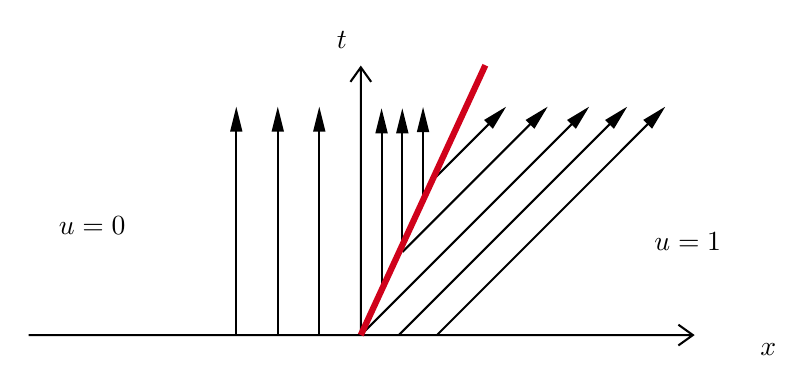
\begin{tikzpicture}[x=0.75pt,y=0.75pt,yscale=-1,xscale=1]
        %uncomment if require: \path (0,187); %set diagram left start at 0, and has height of 187

        %Shape: Axis 2D [id:dp875260399994052] 
        \draw  (120,160) -- (440,160)(280,31) -- (280,160) (433,155) -- (440,160) -- (433,165) (275,38) -- (280,31) -- (285,38)  ;
        %Straight Lines [id:da19535889839268816] 
        \draw    (260,160) -- (260,52) ;
        \draw [shift={(260,50)}, rotate = 450] [fill={rgb, 255:red, 0; green, 0; blue, 0 }  ][line width=0.08]  [draw opacity=0] (12,-3) -- (0,0) -- (12,3) -- cycle    ;
        %Straight Lines [id:da7849799519863265] 
        \draw    (240,160) -- (240,52) ;
        \draw [shift={(240,50)}, rotate = 450] [fill={rgb, 255:red, 0; green, 0; blue, 0 }  ][line width=0.08]  [draw opacity=0] (12,-3) -- (0,0) -- (12,3) -- cycle    ;
        %Straight Lines [id:da6970851759018153] 
        \draw    (220,160) -- (220,52) ;
        \draw [shift={(220,50)}, rotate = 450] [fill={rgb, 255:red, 0; green, 0; blue, 0 }  ][line width=0.08]  [draw opacity=0] (12,-3) -- (0,0) -- (12,3) -- cycle    ;
        %Straight Lines [id:da3176038469211988] 
        \draw    (298.33,160) -- (406.92,51.41) ;
        \draw [shift={(408.33,50)}, rotate = 495] [fill={rgb, 255:red, 0; green, 0; blue, 0 }  ][line width=0.08]  [draw opacity=0] (12,-3) -- (0,0) -- (12,3) -- cycle    ;
        %Straight Lines [id:da4532515514627731] 
        \draw    (316.67,160) -- (425.25,51.41) ;
        \draw [shift={(426.67,50)}, rotate = 495] [fill={rgb, 255:red, 0; green, 0; blue, 0 }  ][line width=0.08]  [draw opacity=0] (12,-3) -- (0,0) -- (12,3) -- cycle    ;
        %Straight Lines [id:da4627175718534131] 
        \draw    (280,160) -- (388.59,51.41) ;
        \draw [shift={(390,50)}, rotate = 495] [fill={rgb, 255:red, 0; green, 0; blue, 0 }  ][line width=0.08]  [draw opacity=0] (12,-3) -- (0,0) -- (12,3) -- cycle    ;
        %Straight Lines [id:da1260105530943243] 
        \draw    (300,114) -- (300,52.83) ;
        \draw [shift={(300,50.83)}, rotate = 450] [fill={rgb, 255:red, 0; green, 0; blue, 0 }  ][line width=0.08]  [draw opacity=0] (12,-3) -- (0,0) -- (12,3) -- cycle    ;
        %Straight Lines [id:da903535329490627] 
        \draw    (300,120) -- (368.59,51.41) ;
        \draw [shift={(370,50)}, rotate = 495] [fill={rgb, 255:red, 0; green, 0; blue, 0 }  ][line width=0.08]  [draw opacity=0] (12,-3) -- (0,0) -- (12,3) -- cycle    ;
        %Straight Lines [id:da9238450729996173] 
        \draw    (315.83,84.17) -- (348.59,51.41) ;
        \draw [shift={(350,50)}, rotate = 495] [fill={rgb, 255:red, 0; green, 0; blue, 0 }  ][line width=0.08]  [draw opacity=0] (12,-3) -- (0,0) -- (12,3) -- cycle    ;
        %Straight Lines [id:da7397791997885115] 
        \draw    (310,95) -- (310,52.17) ;
        \draw [shift={(310,50.17)}, rotate = 450] [fill={rgb, 255:red, 0; green, 0; blue, 0 }  ][line width=0.08]  [draw opacity=0] (12,-3) -- (0,0) -- (12,3) -- cycle    ;
        %Straight Lines [id:da13558321601620804] 
        \draw    (290,136.5) -- (290,52.83) ;
        \draw [shift={(290,50.83)}, rotate = 450] [fill={rgb, 255:red, 0; green, 0; blue, 0 }  ][line width=0.08]  [draw opacity=0] (12,-3) -- (0,0) -- (12,3) -- cycle    ;
        %Straight Lines [id:da2492522635217922] 
        \draw [color={rgb, 255:red, 208; green, 2; blue, 27 }  ,draw opacity=1 ][line width=2.25]    (280,160) -- (340,30) ;

        % Text Node
        \draw (133,101.4) node [anchor=north west][inner sep=0.75pt]    {$u=0$};
        % Text Node
        \draw (420,109.4) node [anchor=north west][inner sep=0.75pt]    {$u=1$};
        % Text Node
        \draw (471,162.4) node [anchor=north west][inner sep=0.75pt]    {$x$};
        % Text Node
        \draw (267,12.4) node [anchor=north west][inner sep=0.75pt]    {$t$};

    \end{tikzpicture}
\end{figure}
\FloatBarrier

Questo è uno \textbf{shock non fisico}. È come se partendo da un punto su una caratteristica e tornando indietro nel tempo potessi ricostruire la linea d'urto. Un po' fidandoci e un po' appellandoci al secondo principio della termodinamica che riguarda l'aumento di entropoia, accettiamo questa denominazione.

\LezioneS{30/03/2021}
\subsection{Condizione di entropia}

Abbiamo risposto al primo quesito, dando un senso al concetto di soluzione quando si presentano discontinuità (grazie alle soluzioni deboli e Rankine-Hugoniot), e dimostrato che l'unicità non è garantita. Ora dobbiamo definire un criterio di selezione che individui possibilmente un'unica soluzione accettabile dal punto di vista del significato fisico del problema.

\emph{Esaminiamo prima un caso ideale:} sia $\displaystyle g' >0,\ q''\geq q''_{\min}  >0$, l'unica soluzione è assegnata dalla formula
\begin{equation}
    G(x,t,u) =u-g(x-q'(u) t) =0
\end{equation}
Grazie al teorema del Dini
\begin{equation*}
    u_{x} =-\frac{G_{x}}{G_{u}} =\frac{g'(x-q'(u) t)}{\underbrace{1+g'(x-q'(u) t) q''(u) t}_{\geq \ g'(x-q'(u) t) q''(u) t}} \leq \frac{1}{q''(u)}\frac{1}{t} \leq \frac{E}{t} \ \ \ \text{dove} \ E=\frac{1}{q''_{\min}}
\end{equation*}
Per il teorema del valor medio, se $\displaystyle x,z\in \mathbb{R} ,\ t >0,z >0\ $
\begin{equation*}
    u(x+z,t) -u(x,t) =u_{x}(\xi _{z,x} ,t) z\leq \frac{E}{t} z
\end{equation*}
Perché questa disuguaglianza valga basta che $u$ sia definita, non è richiesta nessuna regolarità
\begin{definition}
    [Condizione di entropia] Nel caso $q''>0$, la condizione di entropia è rispettata se $\exists E >0$ tale che per ogni $x,z\in \mathbb{R}$, $z>0$ e per ogni $t>0$:
    \begin{equation}
        u(x+z,t) -u(x,t) \leq \frac{E}{t} z
        \label{eq:condizione-di-entropia}
    \end{equation}
\end{definition}
Il nome deriva da una particolare intepretazione fisica valida solo nel modello della dinamica di un gas, dove questa disuguaglianza significa che attraverso la linea di shock l'entropia aumenta.

La \eqref{eq:condizione-di-entropia} ha senso anche per soluzioni discontinue (in particolare, quelle \textbf{deboli}) e non coinvolge operazioni di derivazione. Una soluzione debole che soddisfa la condizione di entropia sarà chiamata \textbf{soluzione entropica.}

Conseguenze:
\begin{itemize}
    \item La funzione
          \begin{equation*}
              x\longmapsto u(x,t) -\frac{E}{t} x,\ t\ \text{fissato}
          \end{equation*}

          è \textbf{non crescente}. Poniamo $\displaystyle x_{2} =x+z,\ x_{1} =x,\ z=x_{2} -x_{1}  >0,\ \text{se} \ x_{2}  >x_{1}$ la \eqref{eq:condizione-di-entropia} diventa
          \begin{equation*}
              u(x_{2} ,t) -u(x_{1} ,t) \leq \frac{E}{t}(x_{2} -x_{1})
          \end{equation*}

          ovvero
          \begin{equation}
              u(x_{2} ,t) -\frac{E}{t} x_{2} \leq u(x_{1} ,t) -\frac{E}{t} x_{1}
              \label{eq:conseguenza-entropia}
          \end{equation}
    \item Per il punto precedente $u$ (essendo monotona) ha solo discontinuità a salto. Inoltre se $\displaystyle (x,t)$ è punto di salto per $u$
          \begin{equation*}
              u_{+}(x,t) < u_{-}(x,t)
          \end{equation*}

          ovvero
          \begin{equation*}
              u(x_{+} ,t) < u(x_{-} ,t)
          \end{equation*}

          Infatti dalla \eqref{eq:conseguenza-entropia} con $\displaystyle x_{1} < x< x_{2}$ facendo tendere $\displaystyle x_{1}\rightarrow x_{-}$ e $\displaystyle x_{2}\rightarrow x_{+}$ si ottiene che il salto è decrescente.
    \item Poiché $\displaystyle q'' >0$, si ha $q'$ strettamente crescente

          \begin{equation*}
              \textcolor[rgb]{0.82,0.01,0.11}{q'(u_{+})} < \textcolor[rgb]{0.25,0.46,0.02}{\frac{q(u_{+}) -q(u_{-})}{u_{+} -u_{-}}} < \textcolor[rgb]{0.29,0.56,0.89}{q'(u_{-})}
          \end{equation*}

          \begin{figure}[htpb]
              \centering
              \tikzset{every picture/.style={line width=0.75pt}} %set default line width to 0.75pt        

              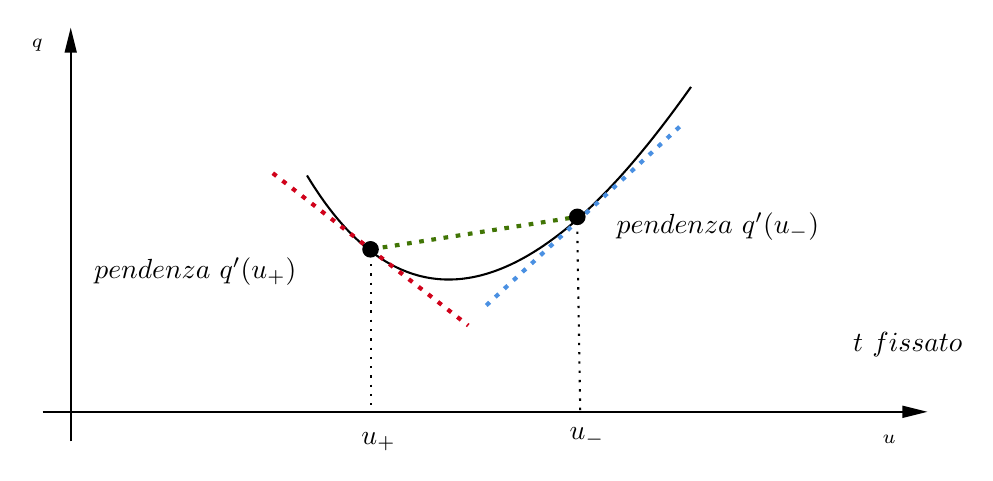
\begin{tikzpicture}[x=0.75pt,y=0.75pt,yscale=-1,xscale=1]
                  %uncomment if require: \path (0,239); %set diagram left start at 0, and has height of 239

                  %Straight Lines [id:da15721075478707136] 
                  \draw    (23.72,195.27) -- (447.97,195.27) ;
                  \draw [shift={(449.97,195.27)}, rotate = 180] [fill={rgb, 255:red, 0; green, 0; blue, 0 }  ][line width=0.08]  [draw opacity=0] (12,-3) -- (0,0) -- (12,3) -- cycle    ;
                  %Straight Lines [id:da5685459692526897] 
                  \draw    (37.24,209.5) -- (37.24,12.25) ;
                  \draw [shift={(37.24,10.25)}, rotate = 450] [fill={rgb, 255:red, 0; green, 0; blue, 0 }  ][line width=0.08]  [draw opacity=0] (12,-3) -- (0,0) -- (12,3) -- cycle    ;
                  %Curve Lines [id:da7633448470292965] 
                  \draw    (151.1,81.41) .. controls (217.51,191.71) and (297.21,93.51) .. (336.11,38.72) ;
                  %Straight Lines [id:da7153295083395204] 
                  \draw  [dash pattern={on 0.84pt off 2.51pt}]  (181.7,124.11) -- (181.7,195.63) ;
                  %Straight Lines [id:da4707175914752779] 
                  \draw  [dash pattern={on 0.84pt off 2.51pt}]  (281.32,108.45) -- (282.74,195.63) ;
                  %Straight Lines [id:da006238229016324315] 
                  \draw [color={rgb, 255:red, 74; green, 144; blue, 226 }  ,draw opacity=1 ][line width=1.5]  [dash pattern={on 1.69pt off 2.76pt}]  (237.44,144.03) -- (332.79,55.91) ;
                  %Straight Lines [id:da29071185698529023] 
                  \draw [color={rgb, 255:red, 208; green, 2; blue, 27 }  ,draw opacity=1 ][line width=1.5]  [dash pattern={on 1.69pt off 2.76pt}]  (134.61,80.29) -- (228.78,153.7) ;
                  %Straight Lines [id:da8603840990839662] 
                  \draw [color={rgb, 255:red, 65; green, 117; blue, 5 }  ,draw opacity=1 ][line width=1.5]  [dash pattern={on 1.69pt off 2.76pt}]  (181.7,116.99) -- (281.32,101.34) ;
                  %Shape: Ellipse [id:dp2153298020546741] 
                  \draw  [draw opacity=0][fill={rgb, 255:red, 0; green, 0; blue, 0 }  ,fill opacity=1 ] (177.7,116.99) .. controls (177.7,114.78) and (179.49,112.99) .. (181.7,112.99) .. controls (183.9,112.99) and (185.7,114.78) .. (185.7,116.99) .. controls (185.7,119.2) and (183.9,120.99) .. (181.7,120.99) .. controls (179.49,120.99) and (177.7,119.2) .. (177.7,116.99) -- cycle ;
                  %Shape: Ellipse [id:dp39414115608124756] 
                  \draw  [draw opacity=0][fill={rgb, 255:red, 0; green, 0; blue, 0 }  ,fill opacity=1 ] (277.32,101.34) .. controls (277.32,99.13) and (279.11,97.34) .. (281.32,97.34) .. controls (283.53,97.34) and (285.32,99.13) .. (285.32,101.34) .. controls (285.32,103.55) and (283.53,105.34) .. (281.32,105.34) .. controls (279.11,105.34) and (277.32,103.55) .. (277.32,101.34) -- cycle ;

                  % Text Node
                  \draw (175.83,203.69) node [anchor=north west][inner sep=0.75pt]  [font=\normalsize]  {$u_{+}$};
                  % Text Node
                  \draw (276.17,201.56) node [anchor=north west][inner sep=0.75pt]  [font=\normalsize]  {$u_{-}$};
                  % Text Node
                  \draw (426.89,204.9) node [anchor=north west][inner sep=0.75pt]  [font=\scriptsize]  {$u$};
                  % Text Node
                  \draw (17.01,14.19) node [anchor=north west][inner sep=0.75pt]  [font=\scriptsize]  {$q$};
                  % Text Node
                  \draw (412.68,155.3) node [anchor=north west][inner sep=0.75pt]  [font=\normalsize]  {$t\ \text{fissato}$};
                  % Text Node
                  \draw (298.82,97.74) node [anchor=north west][inner sep=0.75pt]  [font=\normalsize]  {$\text{pendenza} \ q'(u_{-})$};
                  % Text Node
                  \draw (47.14,119.59) node [anchor=north west][inner sep=0.75pt]  [font=\normalsize]  {$\text{pendenza} \ q'(u_{+})$};

              \end{tikzpicture}
          \end{figure}
          \FloatBarrier

          definiamo \begin{equation*}
              \sigma (u_{+} ,u_{-}) =\textcolor[rgb]{0.25,0.46,0.02}{\frac{q(u_{+}) -q(u_{-})}{u_{+} -u_{-}}}
          \end{equation*}

          ma se $\displaystyle x=s(t)$ è linea d'urto $\displaystyle \sigma (u_{+} ,u_{-}) =\dot{s}(t)$ è la pendenza della retta tangente sulla linea d'urto (ovvero la velocità con cui si muove la discontinuità lungo la linea d'urto) data da Rankine-Hugoniot. Ottengo la \textbf{disuguaglianza dell'entropia}
          \begin{equation*}
              q'(u_{+}) < \dot{s} < q'(u_{-})
          \end{equation*}

          \textbf{La pendenza di una linea d'urto è minore di quella delle caratteristiche che vi arrivano da sinistra e maggiore di quella delle caratteristiche che vi arrivano da destra}: le caratteristiche \textbf{entrano} nella linea d'urto, non è possibile percorrere a ritroso nel tempo una caratteristica e imbattersi in uno shock

          \begin{figure}[htpb]
              \centering
              \tikzset{every picture/.style={line width=0.75pt}} %set default line width to 0.75pt        

              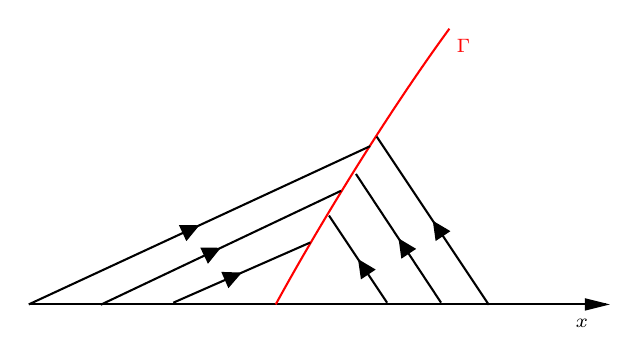
\begin{tikzpicture}[x=0.75pt,y=0.75pt,yscale=-1,xscale=1]
                  %uncomment if require: \path (0,194); %set diagram left start at 0, and has height of 194

                  %Straight Lines [id:da9620336787016928] 
                  \draw    (140,156) -- (418,156) ;
                  \draw [shift={(420,156)}, rotate = 180] [fill={rgb, 255:red, 0; green, 0; blue, 0 }  ][line width=0.08]  [draw opacity=0] (12,-3) -- (0,0) -- (12,3) -- cycle    ;
                  %Curve Lines [id:da25282545301283466] 
                  \draw [color={rgb, 255:red, 255; green, 0; blue, 0 }  ,draw opacity=1 ]   (259,156) .. controls (279.67,118.17) and (312.67,64.17) .. (342.67,23.17) ;
                  %Straight Lines [id:da6910932281248514] 
                  \draw    (284.67,113.17) -- (312.67,155.17) ;
                  \draw [shift={(298.67,134.17)}, rotate = 56.31] [fill={rgb, 255:red, 0; green, 0; blue, 0 }  ][line width=0.08]  [draw opacity=0] (8.93,-4.29) -- (0,0) -- (8.93,4.29) -- cycle    ;
                  %Straight Lines [id:da38448355912897414] 
                  \draw    (297.67,93.17) -- (338.67,155.17) ;
                  \draw [shift={(318.17,124.17)}, rotate = 56.52] [fill={rgb, 255:red, 0; green, 0; blue, 0 }  ][line width=0.08]  [draw opacity=0] (8.93,-4.29) -- (0,0) -- (8.93,4.29) -- cycle    ;
                  %Straight Lines [id:da016088936470342707] 
                  \draw    (307.67,75.17) -- (361.67,156.17) ;
                  \draw [shift={(334.67,115.67)}, rotate = 56.31] [fill={rgb, 255:red, 0; green, 0; blue, 0 }  ][line width=0.08]  [draw opacity=0] (8.93,-4.29) -- (0,0) -- (8.93,4.29) -- cycle    ;
                  %Straight Lines [id:da007455336645831201] 
                  \draw    (275.67,126.17) -- (209.67,155.17) ;
                  \draw [shift={(242.67,140.67)}, rotate = 156.28] [fill={rgb, 255:red, 0; green, 0; blue, 0 }  ][line width=0.08]  [draw opacity=0] (8.93,-4.29) -- (0,0) -- (8.93,4.29) -- cycle    ;
                  %Straight Lines [id:da6406333049601447] 
                  \draw    (290.5,101.25) -- (174.67,156.17) ;
                  \draw [shift={(232.58,128.71)}, rotate = 154.63] [fill={rgb, 255:red, 0; green, 0; blue, 0 }  ][line width=0.08]  [draw opacity=0] (8.93,-4.29) -- (0,0) -- (8.93,4.29) -- cycle    ;
                  %Straight Lines [id:da4848315116268975] 
                  \draw    (304.5,79.75) -- (140,156) ;
                  \draw [shift={(222.25,117.88)}, rotate = 155.13] [fill={rgb, 255:red, 0; green, 0; blue, 0 }  ][line width=0.08]  [draw opacity=0] (8.93,-4.29) -- (0,0) -- (8.93,4.29) -- cycle    ;

                  % Text Node
                  \draw (402,161.4) node [anchor=north west][inner sep=0.75pt]  [font=\scriptsize]  {$x$};
                  % Text Node
                  \draw (344.67,26.57) node [anchor=north west][inner sep=0.75pt]  [font=\scriptsize,color={rgb, 255:red, 255; green, 5; blue, 5 }  ,opacity=1 ]  {$\Gamma $};

              \end{tikzpicture}
          \end{figure}
          \FloatBarrier

\end{itemize}
\begin{nb}
    Nel caso $q''\leq q''_{\max} < 0$ la condizione di entropia diventa
    \begin{equation}
        u(x+z,t) -u(x,t) \geq -\frac{E}{t} z,\quad E=\frac{1}{| q''_{\max}| }
    \end{equation}
    quindi in un punto $(x,t)$ di discontinuità
    \begin{equation*}
        u_{+}(x,t)  >u_{-}(x,t)
    \end{equation*}
    Ma la disuguaglianza d'entropia essendo $q'$ decrescente rimane invariata
\end{nb}
\begin{theorem}
    Se $q\in C^{2}(\mathbb{R})$, strettamente concava o convessa, e $g$ è limitata allora \textbf{esiste unica} la soluzione (integrale, cioè debole) del problema
    \begin{equation}
        \begin{cases}
            u_{t} +q(u)_{x} =0 & x\in \mathbb{R} ,t >0 \\
            u(x,0) =g(x)       & x\in \mathbb{R}
        \end{cases}
        \label{eq:teo-quasi-di-riemann}
    \end{equation}
    \textbf{che soddisfi la condizione di entropia.}
\end{theorem}
Possiamo applicare questo teorema per risolvere il problema \eqref{eq:teo-quasi-di-riemann} con dati al bordo
\begin{equation*}
    g(x) =
    \begin{cases}
        u_{L} , & x< 0 \\
        u_{R} , & x >0
    \end{cases}
\end{equation*}
noto come \textbf{Problema di Riemann}, con $\displaystyle u_{L} \neq u_{R}$ e costanti.

Questo è proprio il caso della coda al semaforo e del traffico a valle, non c'è soluzione classica, ma ce n'è una unica in senso debole che ha senso fisico.
\begin{theorem}
    Sia $q$ strettamente convessa o concava con $\displaystyle q''\geq h >0$ o $\displaystyle q''\leq -h< 0$. Allora l'unica soluzione entropica del problema di Riemann è data da:
    \begin{itemize}
        \item Se $\displaystyle q''\geq h >0$ e $\displaystyle u_{R} < u_{L}$, oppure $\displaystyle q''\leq -h< 0$ e $\displaystyle u_{R}  >u_{L}$

              \textbf{onda d'urto}
              \begin{equation*}
                  u(x,t) =
                  \begin{cases}
                      u_{L} & x< \sigma (u_{L} ,u_{R}) t=s(t) \\
                      u_{R} & x >\sigma (u_{L} ,u_{R}) t=s(t)
                  \end{cases}
              \end{equation*}

              dove
              \begin{equation*}
                  \sigma (u_{L} ,u_{R}) =\dot{s} =\frac{q(u_{R}) -q(u_{L})}{u_{R} -u_{L}} ,\ s(0) =0
              \end{equation*}


        \item Se $\displaystyle q''\geq h >0$ e $\displaystyle u_{R}  >u_{L}$ oppure $\displaystyle q''\leq -h< 0$ e $\displaystyle u_{R} < u_{L}$

              \textbf{onda di rarefazione}
              \begin{equation*}
                  u(x,t) =
                  \begin{cases}
                      u_{L}                     & \frac{x}{t}\leq q'(u_{L})     \\
                      r\left(\frac{x}{t}\right) & q'(u_{L}) < \frac{x}{t}< q'(u_{R}) \\
                      u_{R}                     & \frac{x}{t}\geq q'(u_{R})
                  \end{cases}
              \end{equation*}

              Dove $r(s)=(q')^{-1}(r(s))$ è la funzione inversa di $q'$
    \end{itemize}
\end{theorem}

Prima di fare la dimostrazione esaminiamo i vari casi con dei grafici
\begin{itemize}
    \item Nel caso dell'\textbf{onda d'urto} $\displaystyle \dot{s}$ può essere sia positivo che negativo, assumiamo $\displaystyle \dot{s}$ negativo. Il segno di $\dot{s}$ definisce da che parte si muove la discontinuità.

          \begin{figure}[htpb]
              \centering
              \tikzset{every picture/.style={line width=0.75pt}} %set default line width to 0.75pt        

              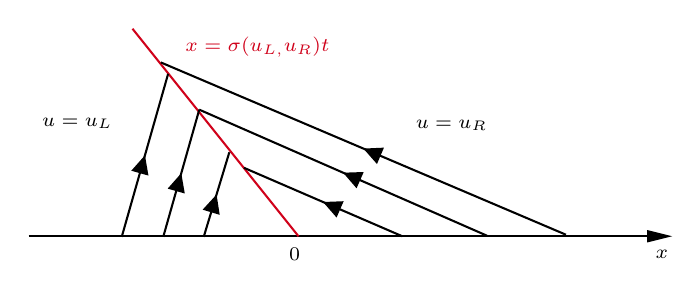
\begin{tikzpicture}[x=0.75pt,y=0.75pt,yscale=-1,xscale=1]
                  %uncomment if require: \path (0,122); %set diagram left start at 0, and has height of 122

                  %Straight Lines [id:da013937525831677622] 
                  \draw    (70,100) -- (108.67,100) -- (378,100) ;
                  \draw [shift={(380,100)}, rotate = 180] [fill={rgb, 255:red, 0; green, 0; blue, 0 }  ][line width=0.08]  [draw opacity=0] (12,-3) -- (0,0) -- (12,3) -- cycle    ;
                  %Straight Lines [id:da204804107678912] 
                  \draw [color={rgb, 255:red, 208; green, 2; blue, 27 }  ,draw opacity=1 ]   (120,0) -- (200,100) ;
                  %Straight Lines [id:da18740730925646099] 
                  \draw [color={rgb, 255:red, 0; green, 0; blue, 0 }  ,draw opacity=1 ]   (173.67,67) -- (250,100) ;
                  \draw [shift={(211.83,83.5)}, rotate = 23.38] [fill={rgb, 255:red, 0; green, 0; blue, 0 }  ,fill opacity=1 ][line width=0.08]  [draw opacity=0] (8.93,-4.29) -- (0,0) -- (8.93,4.29) -- cycle    ;
                  %Straight Lines [id:da7045636842819236] 
                  \draw [color={rgb, 255:red, 0; green, 0; blue, 0 }  ,draw opacity=1 ]   (152.17,39) -- (290.83,99.75) ;
                  \draw [shift={(221.5,69.38)}, rotate = 23.66] [fill={rgb, 255:red, 0; green, 0; blue, 0 }  ,fill opacity=1 ][line width=0.08]  [draw opacity=0] (8.93,-4.29) -- (0,0) -- (8.93,4.29) -- cycle    ;
                  %Straight Lines [id:da32545031002704494] 
                  \draw [color={rgb, 255:red, 0; green, 0; blue, 0 }  ,draw opacity=1 ]   (133.67,16.25) -- (328.83,99.25) ;
                  \draw [shift={(231.25,57.75)}, rotate = 23.04] [fill={rgb, 255:red, 0; green, 0; blue, 0 }  ,fill opacity=1 ][line width=0.08]  [draw opacity=0] (8.93,-4.29) -- (0,0) -- (8.93,4.29) -- cycle    ;
                  %Straight Lines [id:da9013330374285016] 
                  \draw [color={rgb, 255:red, 0; green, 0; blue, 0 }  ,draw opacity=1 ]   (166.67,59.5) -- (154.33,100.25) ;
                  \draw [shift={(160.5,79.88)}, rotate = 106.84] [fill={rgb, 255:red, 0; green, 0; blue, 0 }  ,fill opacity=1 ][line width=0.08]  [draw opacity=0] (8.93,-4.29) -- (0,0) -- (8.93,4.29) -- cycle    ;
                  %Straight Lines [id:da27052016289971936] 
                  \draw [color={rgb, 255:red, 0; green, 0; blue, 0 }  ,draw opacity=1 ]   (152.17,39) -- (134.83,100.25) ;
                  \draw [shift={(143.5,69.63)}, rotate = 105.8] [fill={rgb, 255:red, 0; green, 0; blue, 0 }  ,fill opacity=1 ][line width=0.08]  [draw opacity=0] (8.93,-4.29) -- (0,0) -- (8.93,4.29) -- cycle    ;
                  %Straight Lines [id:da43914600066416565] 
                  \draw [color={rgb, 255:red, 0; green, 0; blue, 0 }  ,draw opacity=1 ]   (137.17,21.75) -- (114.83,100.25) ;
                  \draw [shift={(126,61)}, rotate = 105.88] [fill={rgb, 255:red, 0; green, 0; blue, 0 }  ,fill opacity=1 ][line width=0.08]  [draw opacity=0] (8.93,-4.29) -- (0,0) -- (8.93,4.29) -- cycle    ;

                  % Text Node
                  \draw (144,2.4) node [anchor=north west][inner sep=0.75pt]  [font=\scriptsize,color={rgb, 255:red, 208; green, 2; blue, 27 }  ,opacity=1 ]  {$x=\sigma (u_{L,} u_{R}) t$};
                  % Text Node
                  \draw (75,41.4) node [anchor=north west][inner sep=0.75pt]  [font=\scriptsize]  {$u=u_{L}$};
                  % Text Node
                  \draw (255,42.4) node [anchor=north west][inner sep=0.75pt]  [font=\scriptsize]  {$u=u_{R}$};
                  % Text Node
                  \draw (194,104.4) node [anchor=north west][inner sep=0.75pt]  [font=\scriptsize]  {$0$};
                  % Text Node
                  \draw (370.5,105.4) node [anchor=north west][inner sep=0.75pt]  [font=\scriptsize]  {$x$};

              \end{tikzpicture}
          \end{figure}
          \FloatBarrier

          Fissato $t$, posso avere $\displaystyle u_{R} < u_{L}$ e $q$ convessa $(q''>0)$

          \begin{figure}[htpb]
              \centering
              \tikzset{every picture/.style={line width=0.75pt}} %set default line width to 0.75pt        

              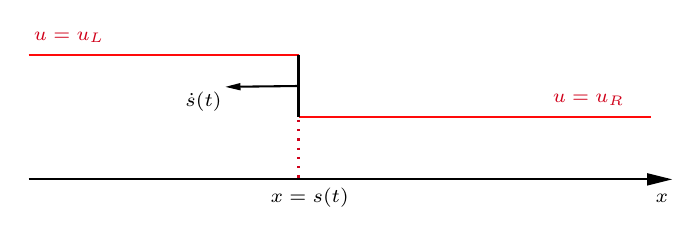
\begin{tikzpicture}[x=0.75pt,y=0.75pt,yscale=-1,xscale=1]
                  %uncomment if require: \path (0,122); %set diagram left start at 0, and has height of 122

                  %Straight Lines [id:da9764488938660592] 
                  \draw    (70,100) -- (378,100) ;
                  \draw [shift={(380,100)}, rotate = 180] [fill={rgb, 255:red, 0; green, 0; blue, 0 }  ][line width=0.08]  [draw opacity=0] (12,-3) -- (0,0) -- (12,3) -- cycle    ;
                  %Straight Lines [id:da37958678944846236] 
                  \draw [color={rgb, 255:red, 255; green, 10; blue, 10 }  ,draw opacity=1 ]   (70,40) -- (200,40) ;
                  %Straight Lines [id:da36304188291259365] 
                  \draw [color={rgb, 255:red, 255; green, 10; blue, 10 }  ,draw opacity=1 ]   (200,70) -- (370,70) ;
                  %Straight Lines [id:da655593479854073] 
                  \draw [color={rgb, 255:red, 208; green, 2; blue, 27 }  ,draw opacity=1 ] [dash pattern={on 0.84pt off 2.51pt}]  (200,40) -- (200,100) ;
                  %Straight Lines [id:da6001360888539051] 
                  \draw    (200,40) -- (200,70) ;
                  %Straight Lines [id:da19326894521279536] 
                  \draw    (200,55) -- (166.83,55.39) ;
                  \draw [shift={(164.83,55.42)}, rotate = 359.32] [fill={rgb, 255:red, 0; green, 0; blue, 0 }  ][line width=0.08]  [draw opacity=0] (7.2,-1.8) -- (0,0) -- (7.2,1.8) -- cycle    ;

                  % Text Node
                  \draw (370.5,105.4) node [anchor=north west][inner sep=0.75pt]  [font=\scriptsize]  {$x$};
                  % Text Node
                  \draw (185,102.4) node [anchor=north west][inner sep=0.75pt]  [font=\scriptsize]  {$x=s(t)$};
                  % Text Node
                  \draw (321,57.4) node [anchor=north west][inner sep=0.75pt]  [font=\scriptsize,color={rgb, 255:red, 208; green, 2; blue, 27 }  ,opacity=1 ]  {$u=u_{R}$};
                  % Text Node
                  \draw (71,27.4) node [anchor=north west][inner sep=0.75pt]  [font=\scriptsize,color={rgb, 255:red, 208; green, 2; blue, 27 }  ,opacity=1 ]  {$u=u_{L}$};
                  % Text Node
                  \draw (144,56.4) node [anchor=north west][inner sep=0.75pt]  [font=\scriptsize]  {$\dot{s}(t)$};

              \end{tikzpicture}
          \end{figure}
          \FloatBarrier

          oppure $\displaystyle u_{R}  >u_{L}$ e $q$ concava $(q''<0)$

          \begin{figure}[htpb]
              \centering
              \tikzset{every picture/.style={line width=0.75pt}} %set default line width to 0.75pt        

              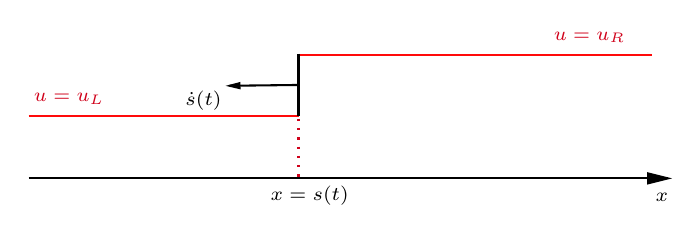
\begin{tikzpicture}[x=0.75pt,y=0.75pt,yscale=-1,xscale=1]
                  %uncomment if require: \path (0,122); %set diagram left start at 0, and has height of 122

                  %Straight Lines [id:da8815235520098277] 
                  \draw    (70,100) -- (378,100) ;
                  \draw [shift={(380,100)}, rotate = 180] [fill={rgb, 255:red, 0; green, 0; blue, 0 }  ][line width=0.08]  [draw opacity=0] (12,-3) -- (0,0) -- (12,3) -- cycle    ;
                  %Straight Lines [id:da059646896144539774] 
                  \draw [color={rgb, 255:red, 255; green, 10; blue, 10 }  ,draw opacity=1 ]   (70,70) -- (200,70) ;
                  %Straight Lines [id:da13412783142262596] 
                  \draw [color={rgb, 255:red, 255; green, 10; blue, 10 }  ,draw opacity=1 ]   (200.5,40.5) -- (370.5,40.5) ;
                  %Straight Lines [id:da19085337118467272] 
                  \draw [color={rgb, 255:red, 208; green, 2; blue, 27 }  ,draw opacity=1 ] [dash pattern={on 0.84pt off 2.51pt}]  (200,40) -- (200,100) ;
                  %Straight Lines [id:da25884047933255006] 
                  \draw    (200,40) -- (200,70) ;
                  %Straight Lines [id:da4742353018370964] 
                  \draw    (200,55) -- (166.83,55.39) ;
                  \draw [shift={(164.83,55.42)}, rotate = 359.32] [fill={rgb, 255:red, 0; green, 0; blue, 0 }  ][line width=0.08]  [draw opacity=0] (7.2,-1.8) -- (0,0) -- (7.2,1.8) -- cycle    ;

                  % Text Node
                  \draw (370.5,105.4) node [anchor=north west][inner sep=0.75pt]  [font=\scriptsize]  {$x$};
                  % Text Node
                  \draw (185,102.4) node [anchor=north west][inner sep=0.75pt]  [font=\scriptsize]  {$x=s(t)$};
                  % Text Node
                  \draw (321.5,27.9) node [anchor=north west][inner sep=0.75pt]  [font=\scriptsize,color={rgb, 255:red, 208; green, 2; blue, 27 }  ,opacity=1 ]  {$u=u_{R}$};
                  % Text Node
                  \draw (71,57.4) node [anchor=north west][inner sep=0.75pt]  [font=\scriptsize,color={rgb, 255:red, 208; green, 2; blue, 27 }  ,opacity=1 ]  {$u=u_{L}$};
                  % Text Node
                  \draw (144,56.4) node [anchor=north west][inner sep=0.75pt]  [font=\scriptsize]  {$\dot{s}(t)$};

              \end{tikzpicture}
          \end{figure}
          \FloatBarrier

          Se $\displaystyle \dot{s}$ è positiva la trattazione è analoga ma la linea di discontinuità si muove verso destra con velocità $\displaystyle \dot{s}(t)$.
    \item Nel caso dell'\textbf{onda di rarefazione} $\displaystyle q'(u_{L}) ,\ q'(u_{R})$ possono essere positivi o negativi, concordi o discordi.

          Supponiamoli \textbf{discordi} e assumiamo $\displaystyle q'(u_{L}) < 0,\ q'(u_{R})  >0$

          \begin{figure}[H]
              \centering
              \tikzset{every picture/.style={line width=0.75pt}} %set default line width to 0.75pt        

              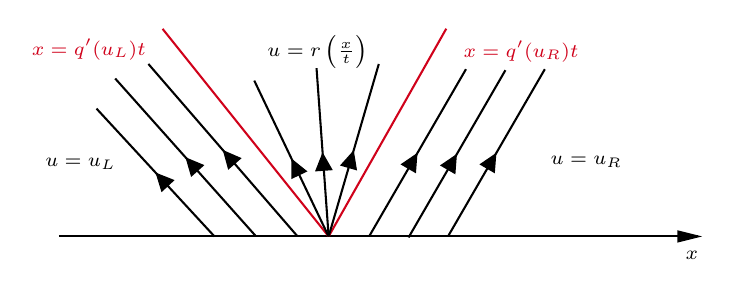
\begin{tikzpicture}[x=0.75pt,y=0.75pt,yscale=-1,xscale=1]
                  %uncomment if require: \path (0,122); %set diagram left start at 0, and has height of 122

                  %Straight Lines [id:da8739094863462447] 
                  \draw    (70,100) -- (378,100) ;
                  \draw [shift={(380,100)}, rotate = 180] [fill={rgb, 255:red, 0; green, 0; blue, 0 }  ][line width=0.08]  [draw opacity=0] (12,-3) -- (0,0) -- (12,3) -- cycle    ;
                  %Straight Lines [id:da5428598737284667] 
                  \draw [color={rgb, 255:red, 208; green, 2; blue, 27 }  ,draw opacity=1 ]   (120,0) -- (200,100) ;
                  %Straight Lines [id:da4689462395847648] 
                  \draw [color={rgb, 255:red, 0; green, 0; blue, 0 }  ,draw opacity=1 ]   (88.17,38.42) -- (145,100) ;
                  \draw [shift={(116.58,69.21)}, rotate = 47.3] [fill={rgb, 255:red, 0; green, 0; blue, 0 }  ,fill opacity=1 ][line width=0.08]  [draw opacity=0] (8.93,-4.29) -- (0,0) -- (8.93,4.29) -- cycle    ;
                  %Straight Lines [id:da011312715740327661] 
                  \draw [color={rgb, 255:red, 0; green, 0; blue, 0 }  ,draw opacity=1 ]   (97.17,23.92) -- (164.83,99.75) ;
                  \draw [shift={(131,61.83)}, rotate = 48.26] [fill={rgb, 255:red, 0; green, 0; blue, 0 }  ,fill opacity=1 ][line width=0.08]  [draw opacity=0] (8.93,-4.29) -- (0,0) -- (8.93,4.29) -- cycle    ;
                  %Straight Lines [id:da8884146928442644] 
                  \draw [color={rgb, 255:red, 0; green, 0; blue, 0 }  ,draw opacity=1 ]   (113.17,16.92) -- (184.83,99.75) ;
                  \draw [shift={(149,58.33)}, rotate = 49.13] [fill={rgb, 255:red, 0; green, 0; blue, 0 }  ,fill opacity=1 ][line width=0.08]  [draw opacity=0] (8.93,-4.29) -- (0,0) -- (8.93,4.29) -- cycle    ;
                  %Straight Lines [id:da87781667555285] 
                  \draw [color={rgb, 255:red, 208; green, 2; blue, 27 }  ,draw opacity=1 ]   (256.67,-0.08) -- (200,100) ;
                  %Straight Lines [id:da4640314644084198] 
                  \draw [color={rgb, 255:red, 0; green, 0; blue, 0 }  ,draw opacity=1 ]   (266.17,19.42) -- (219.5,100) ;
                  \draw [shift={(242.83,59.71)}, rotate = 120.08] [fill={rgb, 255:red, 0; green, 0; blue, 0 }  ,fill opacity=1 ][line width=0.08]  [draw opacity=0] (8.93,-4.29) -- (0,0) -- (8.93,4.29) -- cycle    ;
                  %Straight Lines [id:da4886146876294406] 
                  \draw [color={rgb, 255:red, 0; green, 0; blue, 0 }  ,draw opacity=1 ]   (285.17,19.92) -- (238.5,100.5) ;
                  \draw [shift={(261.83,60.21)}, rotate = 120.08] [fill={rgb, 255:red, 0; green, 0; blue, 0 }  ,fill opacity=1 ][line width=0.08]  [draw opacity=0] (8.93,-4.29) -- (0,0) -- (8.93,4.29) -- cycle    ;
                  %Straight Lines [id:da17132221568371864] 
                  \draw [color={rgb, 255:red, 0; green, 0; blue, 0 }  ,draw opacity=1 ]   (304.17,19.42) -- (257.5,100) ;
                  \draw [shift={(280.83,59.71)}, rotate = 120.08] [fill={rgb, 255:red, 0; green, 0; blue, 0 }  ,fill opacity=1 ][line width=0.08]  [draw opacity=0] (8.93,-4.29) -- (0,0) -- (8.93,4.29) -- cycle    ;
                  %Straight Lines [id:da6152619039020208] 
                  \draw [color={rgb, 255:red, 0; green, 0; blue, 0 }  ,draw opacity=1 ]   (224.17,16.92) -- (200,100) ;
                  \draw [shift={(212.08,58.46)}, rotate = 106.22] [fill={rgb, 255:red, 0; green, 0; blue, 0 }  ,fill opacity=1 ][line width=0.08]  [draw opacity=0] (8.93,-4.29) -- (0,0) -- (8.93,4.29) -- cycle    ;
                  %Straight Lines [id:da05324038437499601] 
                  \draw [color={rgb, 255:red, 0; green, 0; blue, 0 }  ,draw opacity=1 ]   (194.17,18.92) -- (200,100) ;
                  \draw [shift={(197.08,59.46)}, rotate = 85.89] [fill={rgb, 255:red, 0; green, 0; blue, 0 }  ,fill opacity=1 ][line width=0.08]  [draw opacity=0] (8.93,-4.29) -- (0,0) -- (8.93,4.29) -- cycle    ;
                  %Straight Lines [id:da35174962604576] 
                  \draw [color={rgb, 255:red, 0; green, 0; blue, 0 }  ,draw opacity=1 ]   (164.17,24.92) -- (200,100) ;
                  \draw [shift={(182.08,62.46)}, rotate = 64.49] [fill={rgb, 255:red, 0; green, 0; blue, 0 }  ,fill opacity=1 ][line width=0.08]  [draw opacity=0] (8.93,-4.29) -- (0,0) -- (8.93,4.29) -- cycle    ;

                  % Text Node
                  \draw (55.5,3.4) node [anchor=north west][inner sep=0.75pt]  [font=\scriptsize,color={rgb, 255:red, 208; green, 2; blue, 27 }  ,opacity=1 ]  {$x=q'(u_{L}) t$};
                  % Text Node
                  \draw (62,60.9) node [anchor=north west][inner sep=0.75pt]  [font=\scriptsize]  {$u=u_{L}$};
                  % Text Node
                  \draw (305.5,59.9) node [anchor=north west][inner sep=0.75pt]  [font=\scriptsize]  {$u=u_{R}$};
                  % Text Node
                  \draw (370.5,105.4) node [anchor=north west][inner sep=0.75pt]  [font=\scriptsize]  {$x$};
                  % Text Node
                  \draw (263.5,4.4) node [anchor=north west][inner sep=0.75pt]  [font=\scriptsize,color={rgb, 255:red, 208; green, 2; blue, 27 }  ,opacity=1 ]  {$x=q'(u_{R}) t$};
                  % Text Node
                  \draw (169,1.4) node [anchor=north west][inner sep=0.75pt]  [font=\scriptsize]  {$u=r\left(\frac{x}{t}\right)$};

              \end{tikzpicture}
          \end{figure}
          \FloatBarrier

          Fissato $t$, posso avere $\displaystyle u_{R}  >u_{L}$ e $q$ convessa

          \begin{figure}[H]
              \centering
              \tikzset{every picture/.style={line width=0.75pt}} %set default line width to 0.75pt        

              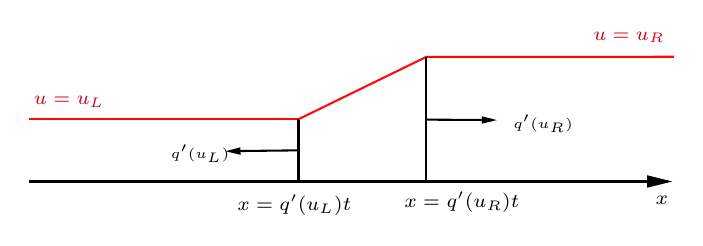
\begin{tikzpicture}[x=0.75pt,y=0.75pt,yscale=-1,xscale=1]
                  %uncomment if require: \path (0,122); %set diagram left start at 0, and has height of 122

                  %Straight Lines [id:da7999736848437151] 
                  \draw    (70,100) -- (378,100) ;
                  \draw [shift={(380,100)}, rotate = 180] [fill={rgb, 255:red, 0; green, 0; blue, 0 }  ][line width=0.08]  [draw opacity=0] (12,-3) -- (0,0) -- (12,3) -- cycle    ;
                  %Straight Lines [id:da305836652713648] 
                  \draw [color={rgb, 255:red, 255; green, 10; blue, 10 }  ,draw opacity=1 ]   (70,70) -- (200,70) ;
                  %Straight Lines [id:da9832604495876003] 
                  \draw [color={rgb, 255:red, 255; green, 10; blue, 10 }  ,draw opacity=1 ]   (261.5,40) -- (381,39.92) ;
                  %Straight Lines [id:da8318436862255643] 
                  \draw    (200,70) -- (200,100) ;
                  %Straight Lines [id:da6832612232516775] 
                  \draw    (200,85) -- (166.83,85.39) ;
                  \draw [shift={(164.83,85.42)}, rotate = 359.32] [fill={rgb, 255:red, 0; green, 0; blue, 0 }  ][line width=0.08]  [draw opacity=0] (7.2,-1.8) -- (0,0) -- (7.2,1.8) -- cycle    ;
                  %Straight Lines [id:da319626835719393] 
                  \draw [color={rgb, 255:red, 255; green, 10; blue, 10 }  ,draw opacity=1 ]   (200,70) -- (261.5,40) ;
                  %Straight Lines [id:da3339460885174421] 
                  \draw    (261.5,40) -- (261.5,100.42) ;
                  %Straight Lines [id:da8426197172623417] 
                  \draw    (261.5,70.21) -- (293.5,70.4) ;
                  \draw [shift={(295.5,70.42)}, rotate = 180.35] [fill={rgb, 255:red, 0; green, 0; blue, 0 }  ][line width=0.08]  [draw opacity=0] (7.2,-1.8) -- (0,0) -- (7.2,1.8) -- cycle    ;

                  % Text Node
                  \draw (370.5,105.4) node [anchor=north west][inner sep=0.75pt]  [font=\scriptsize]  {$x$};
                  % Text Node
                  \draw (169,104.9) node [anchor=north west][inner sep=0.75pt]  [font=\scriptsize]  {$x=q'(u_{L}) t$};
                  % Text Node
                  \draw (340.5,26.4) node [anchor=north west][inner sep=0.75pt]  [font=\scriptsize,color={rgb, 255:red, 208; green, 2; blue, 27 }  ,opacity=1 ]  {$u=u_{R}$};
                  % Text Node
                  \draw (71,57.4) node [anchor=north west][inner sep=0.75pt]  [font=\scriptsize,color={rgb, 255:red, 208; green, 2; blue, 27 }  ,opacity=1 ]  {$u=u_{L}$};
                  % Text Node
                  \draw (137,80.9) node [anchor=north west][inner sep=0.75pt]  [font=\tiny]  {$q'(u_{L})$};
                  % Text Node
                  \draw (249.5,103.4) node [anchor=north west][inner sep=0.75pt]  [font=\scriptsize]  {$x=q'(u_{R}) t$};
                  % Text Node
                  \draw (302,66.4) node [anchor=north west][inner sep=0.75pt]  [font=\tiny]  {$q'(u_{R})$};

              \end{tikzpicture}
          \end{figure}
          \FloatBarrier

          oppure $\displaystyle u_{R} < u_{L}$ e $q$ concava

          \begin{figure}[H]
              \centering
              \tikzset{every picture/.style={line width=0.75pt}} %set default line width to 0.75pt        

              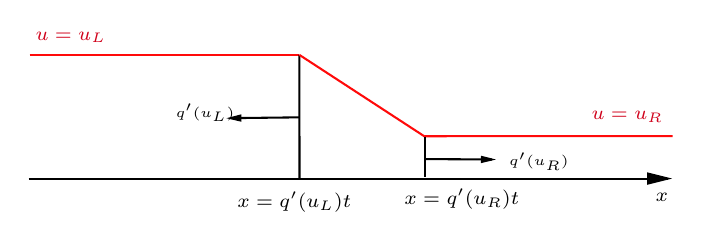
\begin{tikzpicture}[x=0.75pt,y=0.75pt,yscale=-1,xscale=1]
                  %uncomment if require: \path (0,122); %set diagram left start at 0, and has height of 122

                  %Straight Lines [id:da40096426207704594] 
                  \draw    (70,100) -- (378,100) ;
                  \draw [shift={(380,100)}, rotate = 180] [fill={rgb, 255:red, 0; green, 0; blue, 0 }  ][line width=0.08]  [draw opacity=0] (12,-3) -- (0,0) -- (12,3) -- cycle    ;
                  %Straight Lines [id:da28928868833123644] 
                  \draw [color={rgb, 255:red, 255; green, 10; blue, 10 }  ,draw opacity=1 ]   (70.4,40.4) -- (200.4,40.4) ;
                  %Straight Lines [id:da9988430529473442] 
                  \draw [color={rgb, 255:red, 255; green, 10; blue, 10 }  ,draw opacity=1 ]   (260.7,79.6) -- (380.2,79.52) ;
                  %Straight Lines [id:da527024412210664] 
                  \draw    (200.4,40.4) -- (200.47,100.6) ;
                  %Straight Lines [id:da2856018767965278] 
                  \draw    (200.43,70.5) -- (167.27,70.89) ;
                  \draw [shift={(165.27,70.92)}, rotate = 359.32] [fill={rgb, 255:red, 0; green, 0; blue, 0 }  ][line width=0.08]  [draw opacity=0] (7.2,-1.8) -- (0,0) -- (7.2,1.8) -- cycle    ;
                  %Straight Lines [id:da9686181806048182] 
                  \draw [color={rgb, 255:red, 255; green, 10; blue, 10 }  ,draw opacity=1 ]   (200.4,40.4) -- (260.87,79.8) ;
                  %Straight Lines [id:da5056133566064824] 
                  \draw    (260.87,79.8) -- (260.87,99.4) ;
                  %Straight Lines [id:da9953599611024972] 
                  \draw    (261.1,90.61) -- (293.1,90.8) ;
                  \draw [shift={(295.1,90.82)}, rotate = 180.35] [fill={rgb, 255:red, 0; green, 0; blue, 0 }  ][line width=0.08]  [draw opacity=0] (7.2,-1.8) -- (0,0) -- (7.2,1.8) -- cycle    ;

                  % Text Node
                  \draw (370.5,105.4) node [anchor=north west][inner sep=0.75pt]  [font=\scriptsize]  {$x$};
                  % Text Node
                  \draw (169,104.9) node [anchor=north west][inner sep=0.75pt]  [font=\scriptsize]  {$x=q'(u_{L}) t$};
                  % Text Node
                  \draw (339.7,66) node [anchor=north west][inner sep=0.75pt]  [font=\scriptsize,color={rgb, 255:red, 208; green, 2; blue, 27 }  ,opacity=1 ]  {$u=u_{R}$};
                  % Text Node
                  \draw (71.8,27.8) node [anchor=north west][inner sep=0.75pt]  [font=\scriptsize,color={rgb, 255:red, 208; green, 2; blue, 27 }  ,opacity=1 ]  {$u=u_{L}$};
                  % Text Node
                  \draw (139.4,62.5) node [anchor=north west][inner sep=0.75pt]  [font=\tiny]  {$q'(u_{L})$};
                  % Text Node
                  \draw (249.5,103.4) node [anchor=north west][inner sep=0.75pt]  [font=\scriptsize]  {$x=q'(u_{R}) t$};
                  % Text Node
                  \draw (300,86) node [anchor=north west][inner sep=0.75pt]  [font=\tiny]  {$q'(u_{R})$};

              \end{tikzpicture}
          \end{figure}
          \FloatBarrier

          Se invece $q'(u_{L})$ e $q'(u_{R})$ fossero \textbf{concordi} avremmo che le linee vanno nella stessa direzione, ma ciò non causerebbe problemi perché una sarebbe più veloce dell'altra e si creerebbe comunque un ventaglio.
          \begin{figure}[H]
              \centering


              \tikzset{every picture/.style={line width=0.75pt}} %set default line width to 0.75pt        

              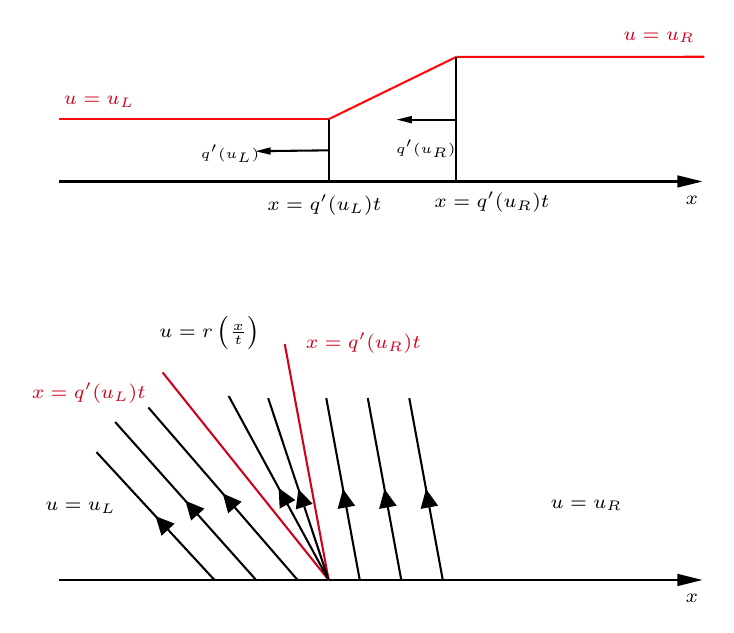
\begin{tikzpicture}[x=0.75pt,y=0.75pt,yscale=-1,xscale=1]
                  %uncomment if require: \path (0,416); %set diagram left start at 0, and has height of 416

                  %Straight Lines [id:da9950736821928572] 
                  \draw    (90,120) -- (398,120) ;
                  \draw [shift={(400,120)}, rotate = 180] [fill={rgb, 255:red, 0; green, 0; blue, 0 }  ][line width=0.08]  [draw opacity=0] (12,-3) -- (0,0) -- (12,3) -- cycle    ;
                  %Straight Lines [id:da9801100467153039] 
                  \draw [color={rgb, 255:red, 255; green, 10; blue, 10 }  ,draw opacity=1 ]   (90,90) -- (220,90) ;
                  %Straight Lines [id:da5156760813370125] 
                  \draw [color={rgb, 255:red, 255; green, 10; blue, 10 }  ,draw opacity=1 ]   (281.5,60) -- (401,59.92) ;
                  %Straight Lines [id:da9368571719365129] 
                  \draw    (220,90) -- (220,120) ;
                  %Straight Lines [id:da07440858746624457] 
                  \draw    (220,105) -- (186.83,105.39) ;
                  \draw [shift={(184.83,105.42)}, rotate = 359.32] [fill={rgb, 255:red, 0; green, 0; blue, 0 }  ][line width=0.08]  [draw opacity=0] (7.2,-1.8) -- (0,0) -- (7.2,1.8) -- cycle    ;
                  %Straight Lines [id:da5705484667972156] 
                  \draw [color={rgb, 255:red, 255; green, 10; blue, 10 }  ,draw opacity=1 ]   (220,90) -- (281.5,60) ;
                  %Straight Lines [id:da7404278798783888] 
                  \draw    (281.5,60) -- (281.5,120.42) ;
                  %Straight Lines [id:da8788990748512959] 
                  \draw    (281.5,90.21) -- (254.86,90.21) ;
                  \draw [shift={(252.86,90.21)}, rotate = 360] [fill={rgb, 255:red, 0; green, 0; blue, 0 }  ][line width=0.08]  [draw opacity=0] (7.2,-1.8) -- (0,0) -- (7.2,1.8) -- cycle    ;
                  %Straight Lines [id:da23323943774510547] 
                  \draw    (90,312) -- (398,312) ;
                  \draw [shift={(400,312)}, rotate = 180] [fill={rgb, 255:red, 0; green, 0; blue, 0 }  ][line width=0.08]  [draw opacity=0] (12,-3) -- (0,0) -- (12,3) -- cycle    ;
                  %Straight Lines [id:da6273394738632234] 
                  \draw [color={rgb, 255:red, 208; green, 2; blue, 27 }  ,draw opacity=1 ]   (140,212) -- (220,312) ;
                  %Straight Lines [id:da5919270574304396] 
                  \draw [color={rgb, 255:red, 0; green, 0; blue, 0 }  ,draw opacity=1 ]   (108.17,250.42) -- (165,312) ;
                  \draw [shift={(136.58,281.21)}, rotate = 47.3] [fill={rgb, 255:red, 0; green, 0; blue, 0 }  ,fill opacity=1 ][line width=0.08]  [draw opacity=0] (8.93,-4.29) -- (0,0) -- (8.93,4.29) -- cycle    ;
                  %Straight Lines [id:da9592585277281807] 
                  \draw [color={rgb, 255:red, 0; green, 0; blue, 0 }  ,draw opacity=1 ]   (117.17,235.92) -- (184.83,311.75) ;
                  \draw [shift={(151,273.83)}, rotate = 48.26] [fill={rgb, 255:red, 0; green, 0; blue, 0 }  ,fill opacity=1 ][line width=0.08]  [draw opacity=0] (8.93,-4.29) -- (0,0) -- (8.93,4.29) -- cycle    ;
                  %Straight Lines [id:da0017728071786706767] 
                  \draw [color={rgb, 255:red, 0; green, 0; blue, 0 }  ,draw opacity=1 ]   (133.17,228.92) -- (204.83,311.75) ;
                  \draw [shift={(169,270.33)}, rotate = 49.13] [fill={rgb, 255:red, 0; green, 0; blue, 0 }  ,fill opacity=1 ][line width=0.08]  [draw opacity=0] (8.93,-4.29) -- (0,0) -- (8.93,4.29) -- cycle    ;
                  %Straight Lines [id:da3876475798196892] 
                  \draw [color={rgb, 255:red, 208; green, 2; blue, 27 }  ,draw opacity=1 ]   (198.86,198.39) -- (220,312) ;
                  %Straight Lines [id:da470433367020763] 
                  \draw [color={rgb, 255:red, 0; green, 0; blue, 0 }  ,draw opacity=1 ]   (218.86,224.39) -- (235,312) ;
                  \draw [shift={(226.93,268.2)}, rotate = 79.56] [fill={rgb, 255:red, 0; green, 0; blue, 0 }  ,fill opacity=1 ][line width=0.08]  [draw opacity=0] (8.93,-4.29) -- (0,0) -- (8.93,4.29) -- cycle    ;
                  %Straight Lines [id:da0014854433931021926] 
                  \draw [color={rgb, 255:red, 0; green, 0; blue, 0 }  ,draw opacity=1 ]   (190.86,224.39) -- (220,312) ;
                  \draw [shift={(205.43,268.2)}, rotate = 71.6] [fill={rgb, 255:red, 0; green, 0; blue, 0 }  ,fill opacity=1 ][line width=0.08]  [draw opacity=0] (8.93,-4.29) -- (0,0) -- (8.93,4.29) -- cycle    ;
                  %Straight Lines [id:da5296522239445665] 
                  \draw [color={rgb, 255:red, 0; green, 0; blue, 0 }  ,draw opacity=1 ]   (171.86,223.39) -- (220,312) ;
                  \draw [shift={(195.93,267.7)}, rotate = 61.49] [fill={rgb, 255:red, 0; green, 0; blue, 0 }  ,fill opacity=1 ][line width=0.08]  [draw opacity=0] (8.93,-4.29) -- (0,0) -- (8.93,4.29) -- cycle    ;
                  %Straight Lines [id:da6700801405222057] 
                  \draw [color={rgb, 255:red, 0; green, 0; blue, 0 }  ,draw opacity=1 ]   (238.86,224.39) -- (255,312) ;
                  \draw [shift={(246.93,268.2)}, rotate = 79.56] [fill={rgb, 255:red, 0; green, 0; blue, 0 }  ,fill opacity=1 ][line width=0.08]  [draw opacity=0] (8.93,-4.29) -- (0,0) -- (8.93,4.29) -- cycle    ;
                  %Straight Lines [id:da46158952227048733] 
                  \draw [color={rgb, 255:red, 0; green, 0; blue, 0 }  ,draw opacity=1 ]   (258.86,224.39) -- (275,312) ;
                  \draw [shift={(266.93,268.2)}, rotate = 79.56] [fill={rgb, 255:red, 0; green, 0; blue, 0 }  ,fill opacity=1 ][line width=0.08]  [draw opacity=0] (8.93,-4.29) -- (0,0) -- (8.93,4.29) -- cycle    ;

                  % Text Node
                  \draw (390.5,125.4) node [anchor=north west][inner sep=0.75pt]  [font=\scriptsize]  {$x$};
                  % Text Node
                  \draw (189,124.9) node [anchor=north west][inner sep=0.75pt]  [font=\scriptsize]  {$x=q'(u_{L}) t$};
                  % Text Node
                  \draw (360.5,46.4) node [anchor=north west][inner sep=0.75pt]  [font=\scriptsize,color={rgb, 255:red, 208; green, 2; blue, 27 }  ,opacity=1 ]  {$u=u_{R}$};
                  % Text Node
                  \draw (91,77.4) node [anchor=north west][inner sep=0.75pt]  [font=\scriptsize,color={rgb, 255:red, 208; green, 2; blue, 27 }  ,opacity=1 ]  {$u=u_{L}$};
                  % Text Node
                  \draw (157,100.9) node [anchor=north west][inner sep=0.75pt]  [font=\tiny]  {$q'(u_{L})$};
                  % Text Node
                  \draw (269.5,123.4) node [anchor=north west][inner sep=0.75pt]  [font=\scriptsize]  {$x=q'(u_{R}) t$};
                  % Text Node
                  \draw (251,98.4) node [anchor=north west][inner sep=0.75pt]  [font=\tiny]  {$q'(u_{R})$};
                  % Text Node
                  \draw (75.5,215.4) node [anchor=north west][inner sep=0.75pt]  [font=\scriptsize,color={rgb, 255:red, 208; green, 2; blue, 27 }  ,opacity=1 ]  {$x=q'(u_{L}) t$};
                  % Text Node
                  \draw (82,272.9) node [anchor=north west][inner sep=0.75pt]  [font=\scriptsize]  {$u=u_{L}$};
                  % Text Node
                  \draw (325.5,271.9) node [anchor=north west][inner sep=0.75pt]  [font=\scriptsize]  {$u=u_{R}$};
                  % Text Node
                  \draw (390.5,317.4) node [anchor=north west][inner sep=0.75pt]  [font=\scriptsize]  {$x$};
                  % Text Node
                  \draw (207.5,191.4) node [anchor=north west][inner sep=0.75pt]  [font=\scriptsize,color={rgb, 255:red, 208; green, 2; blue, 27 }  ,opacity=1 ]  {$x=q'(u_{R}) t$};
                  % Text Node
                  \draw (137,183.4) node [anchor=north west][inner sep=0.75pt]  [font=\scriptsize]  {$u=r\left(\frac{x}{t}\right)$};

              \end{tikzpicture}
          \end{figure}
          \FloatBarrier

\end{itemize}

\begin{dimostrazione}
    Nel caso $\displaystyle q''\geq h >0$
    \begin{itemize}
        \item Poiché abbiamo supposto $q$ convessa siamo nel caso $\displaystyle u_{R} < u_{L}$

              \begin{figure}[H]
                  \centering
                  \tikzset{every picture/.style={line width=0.75pt}} %set default line width to 0.75pt        

                  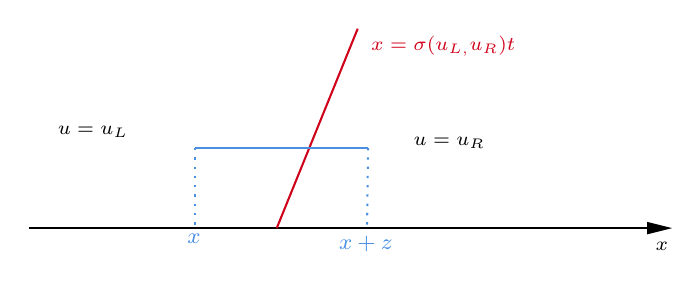
\begin{tikzpicture}[x=0.75pt,y=0.75pt,yscale=-1,xscale=1]
                      %uncomment if require: \path (0,122); %set diagram left start at 0, and has height of 122

                      %Straight Lines [id:da00625345181917103] 
                      \draw    (70,100) -- (378,100) ;
                      \draw [shift={(380,100)}, rotate = 180] [fill={rgb, 255:red, 0; green, 0; blue, 0 }  ][line width=0.08]  [draw opacity=0] (12,-3) -- (0,0) -- (12,3) -- cycle    ;
                      %Straight Lines [id:da8924935270245538] 
                      \draw [color={rgb, 255:red, 208; green, 2; blue, 27 }  ,draw opacity=1 ]   (228.5,3.92) -- (189.5,100) ;
                      %Straight Lines [id:da37864462053275294] 
                      \draw [color={rgb, 255:red, 74; green, 144; blue, 226 }  ,draw opacity=1 ]   (150,61.42) -- (233.5,61.42) ;
                      %Straight Lines [id:da8356896087559171] 
                      \draw [color={rgb, 255:red, 74; green, 144; blue, 226 }  ,draw opacity=1 ] [dash pattern={on 0.84pt off 2.51pt}]  (150,61.42) -- (150,100.42) ;
                      %Straight Lines [id:da18949320614569176] 
                      \draw [color={rgb, 255:red, 74; green, 144; blue, 226 }  ,draw opacity=1 ] [dash pattern={on 0.84pt off 2.51pt}]  (233.5,61.42) -- (233,99.92) ;

                      % Text Node
                      \draw (233.5,5.9) node [anchor=north west][inner sep=0.75pt]  [font=\scriptsize,color={rgb, 255:red, 208; green, 2; blue, 27 }  ,opacity=1 ]  {$x=\sigma (u_{L,} u_{R}) t$};
                      % Text Node
                      \draw (82.5,49.4) node [anchor=north west][inner sep=0.75pt]  [font=\scriptsize]  {$u=u_{L}$};
                      % Text Node
                      \draw (370.5,105.4) node [anchor=north west][inner sep=0.75pt]  [font=\scriptsize]  {$x$};
                      % Text Node
                      \draw (254,54.9) node [anchor=north west][inner sep=0.75pt]  [font=\scriptsize]  {$u=u_{R}$};
                      % Text Node
                      \draw (145,101.4) node [anchor=north west][inner sep=0.75pt]  [font=\footnotesize,color={rgb, 255:red, 74; green, 144; blue, 226 }  ,opacity=1 ]  {$x$};
                      % Text Node
                      \draw (218,102.4) node [anchor=north west][inner sep=0.75pt]  [font=\footnotesize,color={rgb, 255:red, 74; green, 144; blue, 226 }  ,opacity=1 ]  {$x+z$};

                  \end{tikzpicture}
              \end{figure}
              \FloatBarrier

              $u$ è ovviamente soluzione integrale. La condizione di entropia è soddisfatta banalmente per due punti nella zona di sinistra o di destra. Per due punti a cavallo si verifica:
              \begin{equation*}
                  u(x+z,t) -u(x,t) =u_{R} -u_{L} < 0< \frac{E}{t} z
              \end{equation*}
        \item Poiché abbiamo supposto $q$ convessa siamo nel caso $\displaystyle u_{R}  >u_{L}$. La condizione è soddisfatta banalmente nelle zone laterali. Verifichiamo la condizione di entropia all'interno del settore centrale dove $\displaystyle u(x,t) =r\left(\frac{x}{t}\right)$

              Innanzitutto verifichiamo che soddisfa la PDE, ricordando che $r=(q')^{-1}$
              \begin{equation*}
                  u_{t} +q(u)_{x} =-r'\left(\frac{x}{t}\right)\frac{x}{t^{2}} +q'(r) r'\left(\frac{x}{t}\right)\frac{1}{t} =r'\left(\frac{x}{t}\right)\frac{1}{t}\underbrace{\left[ q'(r) -\frac{x}{t}\right]}_{=0} \equiv 0
              \end{equation*}

              Quindi $u$ è soluzione integrale. Per la condizione di entropia
              \begin{align*}
                  u(x+z,t) -u(x,t) & =r\left(\frac{x+z}{t}\right) -r\left(\frac{x}{t}\right)                     &                                  \\
                                   & =r'\left(\frac{\xi _{z,t}}{t}\right)\frac{z}{t} \leq (\text{qualcosa}) & \text{(Teorema del valor medio)}
              \end{align*}

              dove $\displaystyle \xi _{z,t} \in \left(\frac{x}{t} ,\frac{x}{t} +\frac{z}{t}\right)$.

              Per trovare un maggiorante, ricordando che $\displaystyle r=(q')^{-1}$ e usando la regola per la derivata dell'inversa ($r$ è l'inversa di $q'$, quindi $r'$ è la derivata di un'inversa)
              \begin{gather*}
                  r'(s) =\frac{1}{q''(r)} \quad \text{con} \quad s=q'(r) \qquad \Rightarrow \qquad r'(s) \leq \frac{1}{h} \ \text{essendo} \ q''\geq h
              \end{gather*}

              Quindi
              \begin{equation*}
                  r'\left(\frac{\xi _{z,t}}{t}\right)\frac{z}{t} \leq \frac{1}{h}\frac{z}{t} = E \frac{z}{t}
              \end{equation*}

              e la condizione di entropia è soddisfatta con $\displaystyle E=\frac{1}{h}$.
    \end{itemize}

\end{dimostrazione}